\documentclass[conference]{IEEEtran}
\usepackage{cite}
\usepackage{graphicx}
\usepackage{amsmath,amssymb,amsfonts}
\usepackage{algorithmic}
\usepackage{textcomp}
\usepackage{xcolor}
\usepackage{hyperref}
\usepackage{graphicx}
\graphicspath{{figures/}}  % adjust folders as needed
\usepackage{float} % to enable [H] placement
\usepackage[linesnumbered,ruled,vlined]{algorithm2e}



\title{ An End-to-End Multi Agent AI System for Personal Finance: Synthetic Data Generation, Budget Optimization, and Investment Advisory}

\author{
\IEEEauthorblockN{
Aman Jaglan\IEEEauthorrefmark{1},
Smit Pancholi\IEEEauthorrefmark{1},
Nemi Makadia\IEEEauthorrefmark{1},
Yash Doshi\IEEEauthorrefmark{1},
Amir Jafari\IEEEauthorrefmark{2}
}

\IEEEauthorblockA{
\IEEEauthorrefmark{1}Graduate Students, M.S. in Data Science, The George Washington University, Washington, D.C.\\
Emails: \{aman.jaglan, smitsnehal.pancholi, nemi.makadia, yashmanish.doshi\}@gwu.edu
}

\IEEEauthorblockA{
\IEEEauthorrefmark{2}Assistant Professor, Data Science Program, The George Washington University, Washington, D.C.\\
Email: ajafari@gwu.edu
}
}


\begin{document}

\maketitle

\begin{abstract}
Managing personal finances is often complicated by concerns over data privacy and the complexity of financial analysis. This paper presents an end-to-end financial intelligence system comprising three core components: (1) a \textbf{Synthetic Data Generator} that uses Bayesian demographic models and a Conditional GAN to create realistic, individual-level financial transaction datasets; (2) a \textbf{Budget Classification and Optimization module} that includes a classification agent (using logistic regression, LSTM, BERT, and a few-shot LLaMA model) for categorizing spending, and an optimization agent that applies the 50/30/20 budgeting rule through an LLM to suggest adjustments; and (3) an \textbf{LLM-Advisor}, a personalized investment recommendation system that integrates ensemble sentiment analysis (FinBERT, RoBERTa, VADER), fundamental financial metrics, technical indicators (RSI, MACD, moving averages, OBV, ATR), and a GPT-based natural language generation module to deliver practical advice. We detail the system's design and architecture, including diagrams of the data generation pipeline and module interactions. Experimental results show that the synthetic data mirrors real-world patterns, the transaction classification agent achieves approximately 71\% accuracy with a fine-tuned BERT model, and the few-shot LLaMA3-8B-8192 model performs well with human-in-the-loop validation. The optimization agent identifies potential savings of 3--5\% of user income, and the LLM-Advisor synthesizes financial signals into actionable recommendations, achieving sentiment classification accuracy and a stock movement prediction F1 score of up to 0.68. Overall, this work addresses key challenges in personal finance management by offering an integrated system that supports financial literacy, encourages effective budgeting, and helps users make more informed investment decisions.
\end{abstract}
\begin{IEEEkeywords}
Financial Planning, Budget Classification, Budget Optimization, LLaMA 3, Personal Finance AI, Synthetic Data Generation
\end{IEEEkeywords}

\section{Introduction}
Access to individual financial data and effective advisory tools is essential for managing personal finances, yet several challenges remain. Transaction datasets, such as credit card and bank records, are often proprietary and highly sensitive, making it difficult to use them for developing and testing new analytical models. This shortage of available real-world data highlights the need for \textbf{synthetic financial datasets} that can replicate realistic spending behaviors without compromising privacy. At the same time, there is a growing demand for intelligent systems that help individuals understand their spending habits and make informed investment decisions. While traditional approaches like the 50/30/20 budgeting rule \cite{b8} and automated investment platforms (robo-advisors) exist, they typically operate independently and rely on basic rule-based frameworks rather than leveraging the full capabilities of modern AI. This paper aims to bridge these gaps by introducing an integrated AI-based financial intelligence system that spans \textbf{data generation, budget optimization, and investment advisory services}.

The system we propose consists of three interconnected components. First, we develop a \textbf{Synthetic Transaction Data Generator} capable of producing detailed individual-level transaction records. By combining public demographic data, merchant information, Bayesian modeling, and generative adversarial networks, we generate synthetic datasets that closely reflect real-world financial behavior while maintaining user privacy. This enables researchers to train and validate AI models without the need for sensitive personal data. Second, using either synthetic or real transaction data, we build a \textbf{Budget Classification and Optimization module}. This module includes a classification agent that assigns transactions to relevant budget categories such as groceries, travel, and entertainment, along with an optimization agent, powered by a large language model, that provides personalized budgeting suggestions based on widely accepted financial principles.
Third, we introduce an \textbf{LLM-Advisor for investments}, a personalized advisory system that integrates real-time market data, financial news, company fundamentals, and technical indicators. By combining \textbf{sentiment analysis using LLMs}, \textbf{fundamental analysis}, and \textbf{technical analysis}, the advisor generates customized portfolio recommendations along with clear natural language explanations for greater transparency. Together, these components create a comprehensive pipeline: from generating realistic financial data, to training and evaluating models, to delivering AI-powered financial assistance to users.

The rest of this paper is organized as follows: Section II reviews related work in financial data generation and AI-based advisory systems. Section III describes the methodology for synthetic data creation. Section IV outlines the design of the budget classification and optimization agents. Section V presents the architecture and functionality of the LLM-based investment advisor. Section VI concludes the paper by discussing key findings, system contributions, and potential avenues for future work.

\section{Related Work}

\textbf{Synthetic Financial Data Generation:}  
Various methods have been developed to generate synthetic financial data, enabling machine learning research without compromising sensitive user information. Generative Adversarial Networks (GANs) have emerged as a widely used approach for modeling tabular data. For instance, Xu \textit{et al.} proposed the Conditional Tabular GAN (CTGAN), which learns the underlying distribution of real datasets and can synthesize realistic tabular samples \cite{b1}. CTGAN showed strong performance, particularly on datasets with a mix of continuous and categorical features, outperforming traditional statistical techniques. Other GAN-based efforts have focused specifically on financial transactions. Lopez-Rojas \textit{et al.} introduced \textbf{PaySim}, a mobile money transaction simulator designed to generate synthetic datasets for fraud detection research \cite{b2}. PaySim replicates millions of individual transactions based on aggregated real-world patterns, such as those observed in telecommunications data, highlighting a broader trend in related work: using aggregate statistics or patterns as foundations for simulation.

Our approach follows a similar philosophy, utilizing real demographic distributions and merchant data to anchor synthetic transaction generation. Beyond GAN-based methods and simulators, researchers have also explored Bayesian models for financial data synthesis. Probabilistic models offer the advantage of incorporating prior knowledge and quantifying uncertainty during data generation. However, these models often struggle to capture the complex and high-dimensional dependencies inherent in transactional data. To address this, we adopt a hybrid approach that combines the strengths of both paradigms. Bayesian sampling based on demographic distributions to establish a foundation, followed by deep generative modeling with CTGAN to capture more intricate patterns. This hybrid strategy, which blends probabilistic grounding with deep learning, has been explored with limited success in prior studies.


\textbf{Automated Budgeting and Classification:}  
The application of machine learning to personal finance has evolved significantly over the past decade. Early systems relied on rule-based methods and traditional supervised learning models such as Support Vector Machines (SVMs), Decision Trees, and Random Forests, using features such as merchant names, transaction amounts, and locations \cite{hossain2019}. However, these approaches were brittle and struggled with unstructured or ambiguous transaction descriptions. As the complexity of transactional data increased, deep learning techniques, particularly Convolutional Neural Networks (CNNs) and Long Short-Term Memory (LSTM) networks, were introduced to better model sequential dependencies in transaction text \cite{DL}. Although they improved robustness, these models still required large labeled datasets and were sensitive to input variations.

Recent advances in natural language processing have further improved transaction classification. Transformer-based models such as BERT \cite{b6} significantly improved the ability to capture deeper contextual information from merchant names and memo fields. Domain-specific variants, such as FinBERT \cite{finbert2020}, achieved strong results on financial tasks such as sentiment analysis. However, there remains a scarcity of published work on multi-class expense classification, largely due to limited access to labeled financial datasets. To address this, we evaluated a variety of models, including an LSTM and a fine-tuned BERT, trained on synthetic transaction data and enriched merchant descriptions sourced from the Yelp dataset \cite{yelpdata2023}, thus improving generalization to diverse real-world transactions. In addition, we explore a few-shot approach using the LLaMA3-8B-8192 model with custom prompts, where human-in-the-loop feedback further enhanced classification performance. Among all methods, the few-shot LLaMA model achieved the strongest results, illustrating the power of prompt-based learning in low-resource financial classification tasks.

\textbf{Budget Optimization:}  
In the area of personal finance, budgeting heuristics such as the \textbf{50/30/20 rule} \cite{b8} have been proposed to guide spending habits, suggesting that individuals allocate 50\% of their income to needs, 30\% to discretionary expenses, and 20\% to savings. Popularized by Warren and Tyagi \cite{b8}, this rule offers a simple and practical baseline for managing finances. In our system, we integrate this heuristic into an AI agent capable of interactive dialogue with users, blending rule-based spending thresholds with personalized generative advice. To the best of our knowledge, the use of a large language model (LLM) to deliver individualized budgeting recommendations based directly on the transaction data of the user represents a novel combination of traditional financial planning principles and modern AI-driven conversational systems.

\textbf{AI-Powered Investment Advisors:}  
The emergence of robo-advisors has made algorithmic portfolio management widely accessible to consumers. However, traditional robo-advisors primarily rely on modern portfolio theory and often neglect unstructured data sources such as news articles and social media sentiment. Within the financial NLP field, \textbf{sentiment analysis} has been extensively studied as a predictor of market behavior. Financial domain-specific models like \textbf{FinBERT} \cite{b3} have demonstrated superior accuracy in classifying news sentiment compared to general-purpose models. In parallel, general transformers like RoBERTa \cite{b4} offer robust language understanding capabilities that complement finance-focused models. Lexicon-based tools such as \textbf{VADER} have also proven highly effective, particularly for analyzing social media content; in fact, VADER has achieved sentiment classification F1 scores exceeding human performance in some domains (F1=0.96 vs. 0.84 on tweet sentiment \cite{b5}). Ensemble approaches that combine multiple sentiment analysis methods can produce more reliable signals by mitigating individual model biases.

Previous research has also explored blending fundamental analysis (e.g., financial ratios) with textual sentiment analysis for stock prediction, and incorporating technical indicators (such as momentum, moving averages) to improve trading strategies. Building on these foundations, our LLM-Advisor integrates \textbf{news sentiment, fundamental metrics, and technical trends} within a unified framework. Furthermore, we personalize recommendations based on the user’s risk profile—an aspect traditionally handled by simple questionnaires in existing robo-advisory systems.

Recent advances in large language models, including the use of GPT-3 for generating financial insights and analyst-style reports, have further expanded possibilities. The development of finance-specific LLMs such as BloombergGPT \cite{b7} has shown that domain-tuned models can significantly outperform general models on financial tasks. This observation motivates our design, where we leverage a GPT-based module to generate clear and intuitive natural language explanations for the system’s recommendations. By synthesizing these innovations, our LLM-Advisor offers not only data-driven investment suggestions but also \textbf{transparent explanations} for its decisions, helping bridge the gap between quantitative modeling and user trust in AI systems.

To provide an overview of our end-to-end platform, we present the complete system architecture in Figure~\ref{fig:overall-architecture}. The diagram illustrates how the three major components—synthetic data generation, budget classification and optimization, and investment advisory—are integrated into a seamless pipeline. It details the flow of inputs, including user transactions, demographic information, and market data, as well as the interactions between modules and the generation of outputs such as budgetary recommendations and personalized investment advice. 

\begin{figure*}[htbp]
    \centering
    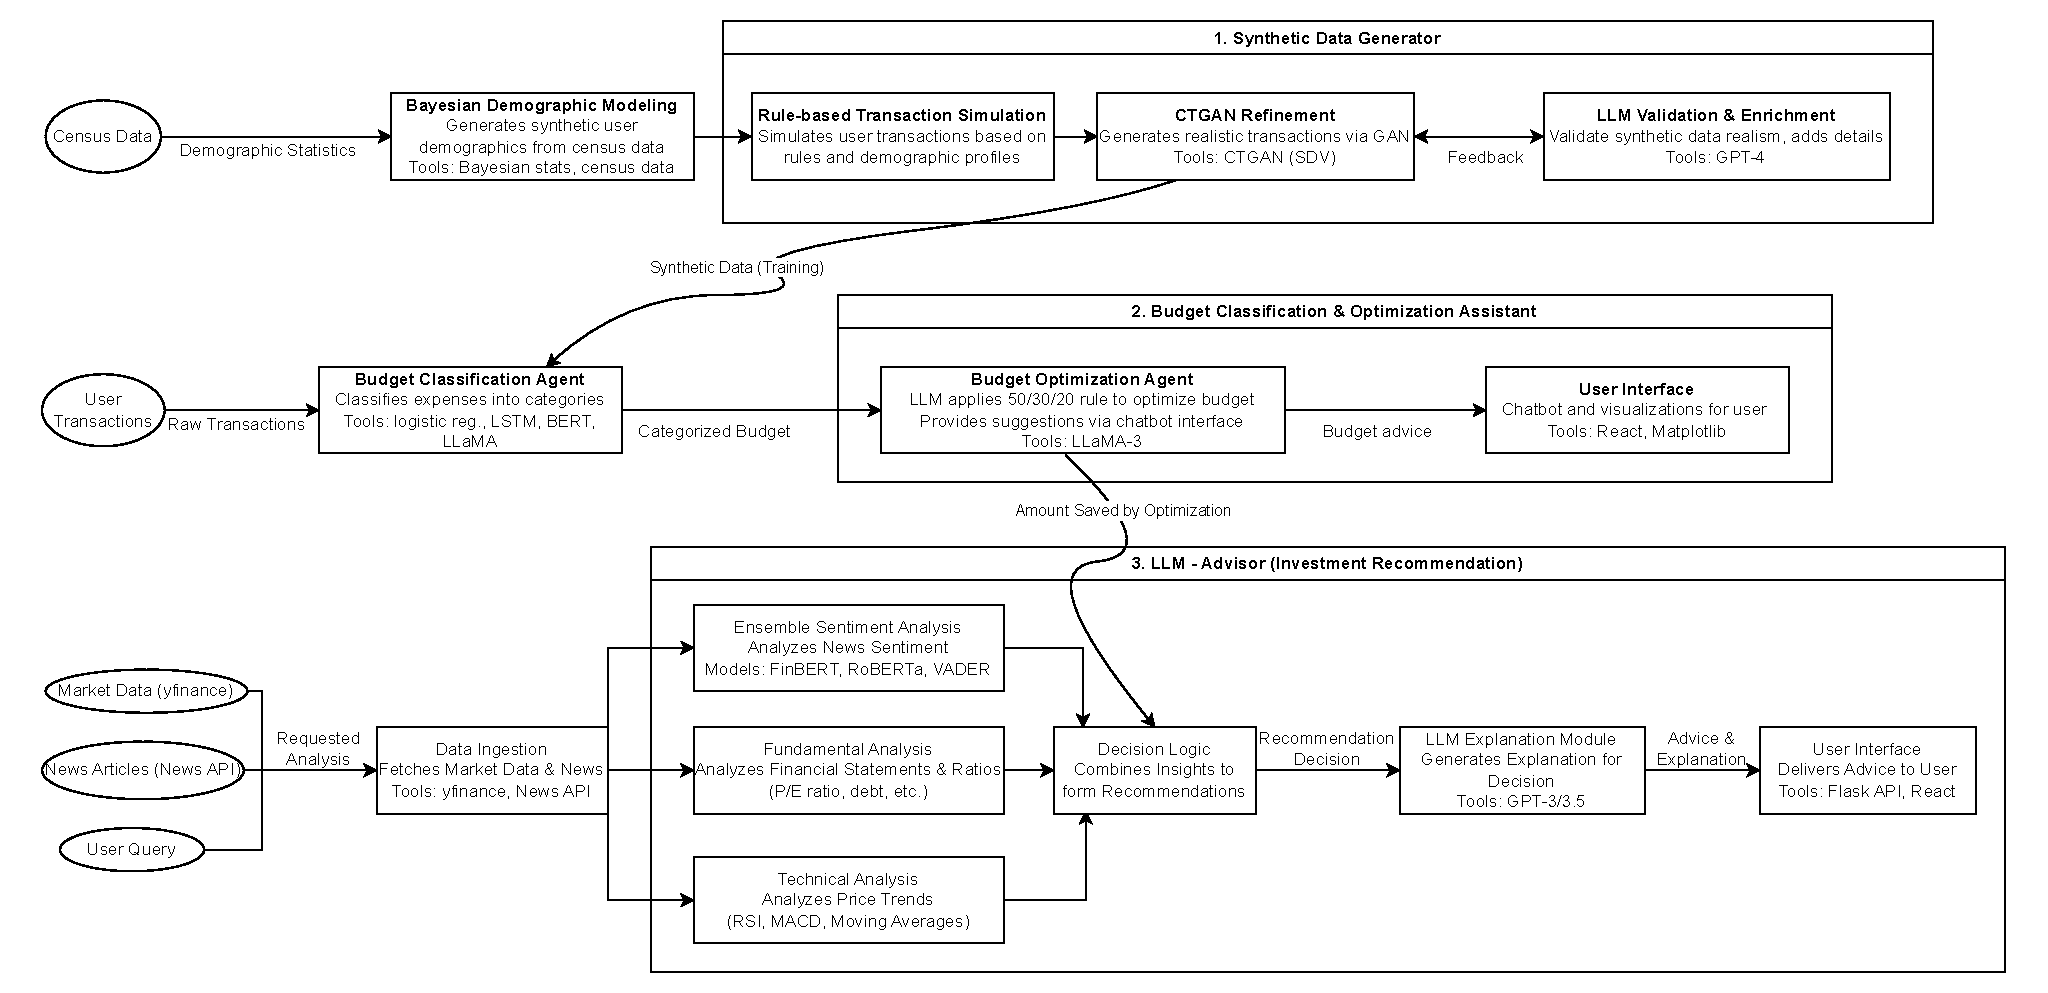
\includegraphics[width=\textwidth]{Overall.pdf}

    \caption{System-wide architecture showing the three major components: (1) Synthetic Data Generator, (2) Budget Classification and Optimization Assistant, and (3) LLM-Advisor for Investment Recommendations. This diagram illustrates the flow of data and logic between modules including input sources (market data, user queries, transactions), intermediate analysis modules (sentiment, fundamental, technical), and the delivery of financial recommendations via an interactive user interface.}

        \label{fig:overall-architecture}
\end{figure*}

\section{Multi-Stage Synthetic Data Generation System}
Our synthetic transaction data generation pipeline is structured into five stages, each designed to progressively increase realism and utility: (1) Bayesian demographic modeling~\cite{acsdata}, (2) rule-based transaction simulation~\cite{paysim2016}, (3) GAN-based refinement~\cite{ctgan2019}, (4) LLM-driven enrichment~\cite{brown2020}, and (5) a hybrid feedback loop that iteratively combines outputs. Each stage targets a distinct aspect of complexity—demographic modeling ensures macro-level statistical accuracy~\cite{acsdata}, rule-based logic captures domain-specific behavior~\cite{paysim2016}, GANs model intricate statistical dependencies~\cite{ctgan2019}, and LLMs enhance semantic richness~\cite{brown2020}. The final hybrid stage integrates these improvements to produce coherent, realistic transaction records. Figure~\ref{fig:pipeline} illustrates the complete architecture, from demographic inputs to finalized transactions. We describe each stage in more detail below.



\subsection{Bayesian Demographic Modeling} 
We begin by generating a synthetic population of customers (or households) using a Bayesian demographic model grounded in real-world data~\cite{acsdata}. Publicly available demographic statistics (e.g., census aggregates) at the geographic level of ZIP codes serve as the foundation~\cite{acsdata}. Each region provides aggregate counts of households broken down by attributes such as age bracket, income range, household size, number of earners, and marital status. We treat these aggregates as probability distributions from which individual household profiles can be sampled. Specifically, if \( N_{z,i} \) denotes the number of households of type \( i \) in region \( z \), the probability that a sampled household has profile \( i \) is defined as:
\begin{equation}
P(\text{profile}=i \mid \text{region}=z) = \frac{N_{z,i}}{\sum_j N_{z,j}}~.
\label{eq:bayes-demo}
\end{equation}
This sampling strategy ensures that the synthetic microdata reflects observed macro-level demographic distributions.

In practice, for each region, we iterate through demographic sub-categories (e.g., age brackets) and generate the appropriate number of synthetic households matching those characteristics. Additional attributes are assigned conditionally: after fixing an age bracket, we sample other features such as marital status or number of earners based on their observed conditional distributions within that subgroup. The output of this stage is a synthetic customer database that captures realistic demographic variability.



% Mathematical formulation of Bayesian demographic model
Given demographic features \( x \), the income \( y \) is modeled as:
\[
y \sim \mathcal{N}(\mu(x), \sigma^2(x))
\]
where \( \mu(x) \) and \( \sigma^2(x) \) are estimated using Bayesian regression. The posterior over parameters \( \theta \) is:
\[
P(\theta \mid D) \propto P(D \mid \theta) P(\theta)
\]
Synthetic samples are drawn from the posterior predictive:
\[
\hat{y} \sim \int P(y \mid x, \theta) P(\theta \mid D) d\theta
\]

\begin{table}[htbp]
\centering
\caption{Demographic Snapshot for Zipcode 20001}
\begin{tabular}{|l|r|}
\hline
\textbf{Feature} & \textbf{Value} \\
\hline
Total Households & 23,831 \\
Households Age 25–44 & 14,460 \\
Married-couple Families & 4,860 \\
Female Householders (no spouse) & 1,562 \\
2-person Families & 4,320 \\
1 Earner Households & 1,263 \\
White Householders (\%) & 54.5 \\
Black Householders (\%) & 26.8 \\
\hline
\end{tabular}
\label{tab:demographics_20001}
\end{table}

\subsection{Rule-Based Transaction Simulation}
Building on the synthetic population generated in Stage 1, Stage 2 simulates financial transactions for each synthetic customer using a rule-based approach~\cite{paysim2016}. Domain knowledge and heuristic assumptions are incorporated to emulate realistic spending behaviors~\cite{paysim2016}. Each synthetic customer is first assigned a personalized monthly spending profile across various expense categories (e.g., groceries, utilities, entertainment), calibrated according to their income level and household characteristics. For example, higher-income households typically exhibit larger overall monthly expenditures with greater allocations toward discretionary categories such as travel and luxury goods, whereas lower-income households allocate a larger share of their budget to essentials.

Based on this profile, we simulate individual transactions. For each customer \( i \), a fixed number of transactions (e.g., 30 per month) is generated to represent typical monthly activity. For each transaction, a category \( c \) is selected from the customer’s spending profile, and the transaction amount \( a \) is sampled as a fraction of the allocated monthly budget for that category. Specifically, if \( B_i(c) \) denotes the monthly budget for category \( c \) assigned to customer \( i \), a random fraction \( r \sim \mathrm{Uniform}(0.05, 0.30) \) is drawn, and the transaction amount is computed as:
\begin{equation}
a = B_i(c) \times r~,
\label{eq:txn-amount}
\end{equation}
ensuring that individual purchases represent a plausible proportion of the monthly allocation.

Each transaction is further assigned a timestamp, sampled uniformly over a recent time window (e.g., the past 30 days), and a merchant identifier. Merchant selection prioritizes contextual plausibility: the simulator first attempts to assign a merchant operating within the same category and geographic area (based on ZIP code) as the customer. If no local match is available, a generic or randomly selected merchant is used instead. This rule-based simulation process produces an initial synthetic transaction dataset \( D_0 \), which captures realistic spending patterns and temporal dynamics. However, \( D_0 \) may not yet fully replicate the complex correlations observed in real-world financial transaction datasets.



\subsection{GAN-Based Data Refinement} 
In Stage 3, we enhance the realism of the synthetic transactions by applying a generative adversarial network (GAN) specialized for tabular data~\cite{ctgan2019}. Specifically, we use a CTGAN model (Conditional Tabular GAN) to learn complex, higher-dimensional statistical relationships from the Stage 2 simulated transactions, supplemented with any available real-world data. The CTGAN consists of a generator \( G \) and a discriminator \( D \) trained on the dataset \( D_0 \). The training objective follows the standard minimax formulation:
\begin{equation}
\min_{G} \max_{D} V(D, G) = 
\mathbb{E}_{x \sim p_{\text{data}}}[\log D(x)] +
\mathbb{E}_{z \sim p(z)}[\log(1 - D(G(z)))]
\label{eq:gan-loss}
\end{equation}
where \( p_{\text{data}} \) represents the distribution of the training data (here, the Stage 2 output \( D_0 \)), and \( p(z) \) denotes the prior over latent variables (e.g., a uniform noise vector).

In practice, we train the CTGAN for a fixed number of epochs (e.g., 100) using the open-source implementation from the Synthetic Data Vault (SDV) library~\cite{ctgan2019}. CTGAN is particularly well-suited for mixed-type datasets, transforming categorical columns via conditional one-hot encoding to better capture relationships such as merchant category frequencies. Once trained, the generator \( G \) can produce an arbitrary number of new transactions. We denote the set of \( m \) synthetic transactions generated during iteration \( k \) as \( S^{(k)} = \{x_1, x_2, \ldots, x_m\} \) (for example, \( m=5000 \) samples in the first iteration).

The transactions generated by CTGAN introduce additional variability and capture subtler patterns that may not have been explicitly modeled in Stage 2. For instance, the CTGAN can learn to generate more realistic variation in transaction amounts or reflect subtle correlations, such as the association between specific merchants and purchase categories or between customer attributes and spending behaviors. However, since the GAN is purely data-driven, it can also generate implausible or unrealistic transactions that violate domain-specific constraints—this motivates the subsequent refinement stage.


\begin{table}[H]
\centering
\small
\renewcommand{\arraystretch}{1.3}
\caption{Sample Customers Generated by GAN}
\label{tab:gan_customers}
\resizebox{\linewidth}{!}{ % Resize to full text width
\begin{tabular}{|l|c|c|c|c|c|c|}
\hline
\textbf{ID} & \textbf{Zip} & \textbf{Age} & \textbf{Status} & \textbf{Size} & \textbf{Income} & \textbf{Gender} \\
\hline
\texttt{0bed...376a} & 20019 & 62 & Single  & 2 & \$56,221  & Female \\
\hline
\texttt{d0a1...87ce} & 20010 & 24 & Single  & 3 & \$76,289  & Female \\
\hline
\texttt{4076...7e12} & 20009 & 61 & Married & 3 & \$144,933 & Male   \\
\hline
\end{tabular}
}
\end{table}




\begin{table*}[htbp]
\centering
\small
\renewcommand{\arraystretch}{1.3}
\caption{Sample Transactions Generated by CTGAN}
\label{tab:ctgan_transactions}
\begin{tabular}{|l|c|c|l|r|}
\hline
\textbf{User ID} & \textbf{Zip} & \textbf{Category} & \textbf{Merchant} & \textbf{Amount (\$)} \\
\hline
\texttt{2478...4294c}   & 20006 & Groceries     & Vidol Luffon LLC     & 360.62 \\
\hline
\texttt{dbc1...fd99}    & 20004 & Dining        & Jasmines Hair Gallery & 148.09 \\
\hline
\texttt{3f83...e03e04}  & 20001 & Personal Care & CHURCH DC LLC.        & 167.71 \\
\hline
\end{tabular}
\end{table*}





\subsection{LLM-Based Data Enrichment and Validation} 
Stage 4 introduces a knowledge-driven validation layer by utilizing a large language model (LLM) accessed via an API to enrich and verify the synthetic transactions~\cite{brown2020}. The objective at this stage is to embed semantic context into the data and filter out implausible records. We integrate an LLM (such as OpenAI's GPT-4) as an oracle capable of analyzing transaction details and providing feedback or additional attributes.

For each transaction \( x \) produced by the CTGAN, we construct a prompt summarizing the relevant customer profile attributes alongside transaction-specific fields such as merchant, category, and amount. This prompt is then submitted to the LLM, which returns an enriched version of the transaction, denoted as \( x' = f_{\text{LLM}}(x) \). The enrichment may include new annotations; for example, the LLM can generate a \textit{fraud likelihood score}—a numerical indicator (between 0 and 1) estimating how typical or suspicious the transaction appears based on learned financial patterns. The LLM may also correct inconsistencies, such as mismatches between the merchant name and transaction category, or add a brief descriptive label for additional semantic context.

These LLM-generated attributes, such as the fraud risk score \( f_{\text{LLM}}(x) \), are appended to the synthetic transaction record. To further improve dataset quality, we apply a filtering criterion: transactions with fraud scores exceeding a threshold \( \tau \) (e.g., \( \tau = 0.8 \)) are excluded from the final dataset. Formally, for each batch of generated transactions \( S^{(k)} \), we retain only the subset satisfying:
\begin{equation}
S_{\text{valid}}^{(k)} = \{ x \in S^{(k)} : f_{\text{LLM}}(x) < \tau \},
\label{eq:llm-filter}
\end{equation}
where \( S_{\text{valid}}^{(k)} \) contains only those records deemed plausible by the LLM.

This enrichment step acts as a domain-informed post-processing filter, adding qualitative, knowledge-based validation that purely statistical methods may overlook. The output of this stage is a curated set of enriched and vetted synthetic transactions ready for downstream integration. Table~\ref{tab:example-txns} provides an example of an enriched synthetic transaction, showing both the original fields (customer attributes, merchant, category, amount) and the LLM-generated fraud risk score, demonstrating how LLM insights directly enhance dataset credibility.



\begin{figure}[htbp]
\centering
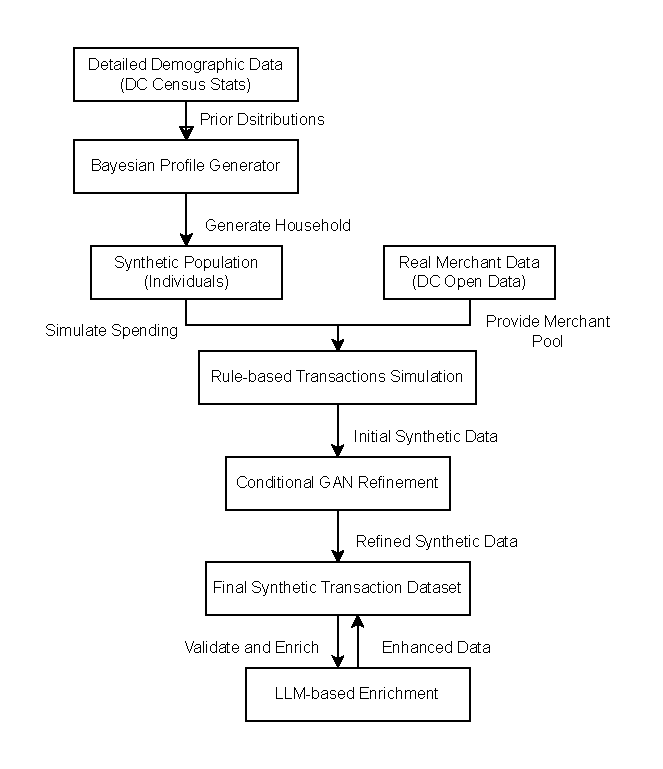
\includegraphics[width=\linewidth]{SynData.pdf}
\caption{Pipeline Diagram: Multi-stage synthetic transaction generation system integrating demographic modeling, GAN refinement, and LLM-based enrichment.}
\label{fig:pipeline}
\end{figure}

\begin{table*}[htbp]
\centering
\small
\renewcommand{\arraystretch}{1.3}
\caption{Sample Customers Generated by LLM}
\label{tab:deepseek_customers}
\begin{tabular}{|l|c|c|c|c|c|c|}
\hline
\textbf{ID} & \textbf{Zip} & \textbf{Age} & \textbf{Status} & \textbf{Size} & \textbf{Income} & \textbf{Gender} \\
\hline
\texttt{2a35...87ad} & 20001 & 20 & Single  & 2 & \$120,000 & Female \\
\hline
\texttt{3162...6508} & 20001 & 30 & Married & 3 & \$150,000 & Female \\
\hline
\texttt{2144...a83}  & 20001 & 45 & Married & 4 & \$160,000 & Male   \\
\hline
\end{tabular}
\end{table*}





\subsection{Hybrid Integration and Iterative Feedback Loop}
In the final stage, we introduce a feedback mechanism by reintegrating the LLM-validated synthetic data back into the generative process, creating an iterative refinement loop~\cite{brown2020}. The objective is to enable the CTGAN to gradually internalize the LLM's feedback over multiple cycles, thereby enhancing the overall quality and plausibility of the generated data.

We begin with the initial dataset \( D_0 \), composed of rule-based simulated transactions (and any available real data). Following the first round of GAN-based refinement (Stage 3) and LLM-based validation (Stage 4), we obtain a set of high-quality synthetic transactions \( S_{\text{valid}}^{(1)} \). These validated transactions are then added to the training set. After the first iteration (\( k = 1 \)), the updated dataset is:
\begin{equation}
D_{1} = D_{0} \cup S_{\text{valid}}^{(1)}~,
\label{eq:augment}
\end{equation}
where \( D_1 \) now includes both the original and the newly validated synthetic samples. The CTGAN is retrained on \( D_1 \), completing one cycle of feedback. 

This iterative process is repeated for a fixed number of cycles or until performance convergence is observed. In each iteration \( k \), the generator \( G \) progressively improves its ability to produce synthetic transactions that satisfy the LLM's semantic constraints, while the LLM continues to validate and enrich new outputs. The pseudo-code for this hybrid training loop is outlined in Algorithm~\ref{alg:hybrid}. 

In our experiments, we found that 2--3 cycles were sufficient for the CTGAN to internalize most of the domain knowledge enforced by the LLM, resulting in a generator capable of producing highly plausible transactions without excessive reliance on external validation. After completing the iterative training, a final batch of synthetic transactions is generated using the updated CTGAN, with one last round of LLM enrichment applied to ensure consistency. The final output is an enhanced synthetic transaction dataset that combines statistical realism with semantic integrity.



\begin{algorithm}[t]
\caption{Hybrid CTGAN+LLM Training Loop for Synthetic Transactions}
\label{alg:hybrid}
\small
\SetAlgoLined
\KwIn{Initial dataset $D_0$, LLM threshold $\tau$, number of cycles $N$}
\KwOut{Trained CTGAN generator $G$}
Train CTGAN $G$ on $D_0$\;
\For{$k \leftarrow 1$ \KwTo $N$}{
    $S^{(k)} \leftarrow G.\text{generate}(m)$ samples\;
    Enrich each $x \in S^{(k)}$ via LLM to get $f_{\text{LLM}}(x)$\;
    $S_{\text{valid}}^{(k)} \leftarrow \{ x \in S^{(k)} : f_{\text{LLM}}(x) < \tau \}$\;
    $D_k \leftarrow D_{k-1} \cup S_{\text{valid}}^{(k)}$\;
    Retrain $G$ on $D_k$\;
}
\end{algorithm}


\begin{table*}[htbp]
\centering
\small
\renewcommand{\arraystretch}{1.3}
\caption{Sample Transactions Generated by Hybrid Model}
\label{tab:hybrid_transactions}
\begin{tabular}{|r|c|l|l|c|}
\hline
\textbf{Amount (\$)} & \textbf{Date} & \textbf{Merchant Name} & \textbf{Category} & \textbf{Payment Type} \\
\hline
43.92  & 2024-03-16 & SIAM HOUSE DC INC. & Restaurant Dining & Credit Card \\
\hline
23.50  & 2024-03-16 & APRA ONE CORP & Restaurant Dining & Credit Card \\
\hline
85.99  & 2024-11-20 & UNIVERSITY OF THE DISTRICT OF COLUMBIA (UDC) & Catering Services & Credit \\
\hline
145.67 & 2024-11-20 & Target Corporation & Grocery Store & Credit Card \\
\hline
\end{tabular}
\end{table*}



\subsection{Synthetic Data Evaluation}
We conducted a qualitative evaluation to assess the fidelity and usefulness of the synthetic dataset~\cite{eaves2024}. Key aggregate characteristics were compared against publicly available statistics for Washington, D.C.~\cite{acsdata}. For example, the distribution of transaction amounts across categories in the synthetic data closely mirrored typical spending patterns—housing-related transactions had the highest average values, while categories like food and groceries appeared more frequently but with moderate amounts. Additionally, the diversity in merchant names and the temporal distribution of transaction timestamps contributed to the dataset’s resemblance to actual financial records.

To identify potential artifacts introduced by the generative model, we manually inspected the data for anomalies. Notably, the CTGAN did not produce implausible values such as negative amounts or invalid dates~\cite{ctgan2019}. It even introduced natural variability that had not been explicitly encoded in the rule-based simulation—for instance, some individuals exhibited irregular spending patterns, indicating that the model was able to reflect deviations from average financial behavior. One observed limitation is that extremely rare or outlier behaviors may be underrepresented, particularly if they were not present in the initial simulation data or were insufficiently captured during training. However, for our primary objective—training and evaluating classification models—capturing broad and plausible spending patterns was more important than simulating every edge case.

In summary, the synthetic dataset served effectively as a \textbf{proxy for real personal finance data}, enabling the development of downstream components in a privacy-preserving manner. In the following section, we describe how this dataset (or real user data, when available) is used to drive the automated budgeting assistant.





\section{Budget Classification and Optimization Agents}

\subsection{Budget Classification Agent Design}

The classification agent is responsible for automatically assigning a \textbf{spending category} (e.g., Grocery, Travel, Shopping, Utilities) to each transaction—an essential step in constructing a coherent summary of the user's financial activity. To perform this task, we evaluated four modeling strategies with increasing levels of sophistication: (1) a Logistic Regression model based on manually engineered features, (2) a recurrent neural network (LSTM), (3) a fine-tuned BERT transformer, and (4) a few-shot large language model (LLaMA 3) accessed via API. While the first three models were trained on labeled transaction data, the LLaMA model was prompted using example-based instructions. 

The training data was derived from our synthetic data generator, which produces labeled transactions by design—each transaction is generated within a specific category, providing ground-truth labels for supervised learning. To further improve BERT’s ability to generalize to varied merchant names and transaction descriptions, we fine-tuned it using merchant data from the Yelp dataset \cite{yelpdata2023}, which contributed additional linguistic diversity and context. 

We also ensured that the dataset reflected the natural class imbalance commonly found in personal finance data: categories such as “Food” or “Shopping” appear frequently, while others like “Travel” or “Education” are less common. This imbalance was preserved intentionally to better mirror real-world expense distributions and challenge the models under realistic conditions.


The \textbf{Logistic Regression} model served as a natural baseline for our experiments, offering both speed and interpretability. Each transaction was primarily represented by the merchant name text (along with optional features such as merchant category or description, when available). We applied TF-IDF vectorization to the merchant name to generate feature inputs for the classifier. This approach allowed the model to detect obvious keyword-based signals (for example, “Pizza” typically suggesting Restaurant/Food, or “Airlines” implying Travel). However, because Logistic Regression treats words independently without considering contextual relationships, it could misclassify transactions from merchants with ambiguous or less descriptive names.

We next explored using an \textbf{LSTM network} to capture sequential patterns present in merchant names or descriptions. The LSTM processes the character or word sequence associated with each transaction’s merchant name, learning an internal representation that is then used to predict the spending category. In theory, a sequential model like LSTM can recognize meaningful substrings or character-level cues—for example, detecting that the presence of “\emph{Air}” within a longer merchant name may suggest a connection to travel. We employed embedding layers to encode characters or tokens and trained the LSTM end-to-end on the classification task, using a weighted cross-entropy loss to account for class imbalance. 
While the LSTM was better suited to capturing the order and structure of words compared to simpler models, it faced challenges in generalization—particularly for sparse or rarely occurring categories. Given the size of our dataset and the diversity of merchant names, the model often overfitted to specific words it had seen during training rather than learning broader, transferable patterns.

Our third approach involved utilizing \textbf{BERT} \cite{b6} to enhance classification performance by leveraging its deep contextual understanding capabilities. We fine-tuned a pre-trained \texttt{bert-base-uncased} model, adding a classification head to adapt it for our multi-class classification task. Fine-tuning was performed on our Yelp-derived dataset over five epochs using the AdamW optimizer.
BERT, having been pre-trained on massive language corpora, is adept at capturing both contextual meaning and subtle semantic relationships within text. Through fine-tuning, we adapted these generalized representations to the specific demands of our transaction categorization task. For example, BERT was able to associate merchants like “Shell Gas Station” and “ExxonMobil” with fuel purchases, even though their names differ significantly, by relying on its learned contextual embeddings. 
This ability to generalize across varied merchant descriptions improved the robustness of the classification, particularly for ambiguous or less informative merchant names. Additionally, the fine-tuned BERT model substantially improved recall on underrepresented categories, a result attributed to its strong capacity for modeling context across sparse examples.


Finally, we explored a prompt-based classification approach using a large language model accessed via an API, specifically \textbf{LLaMA 3} provided by Groq \cite{groqllama2024}. Rather than training a model from scratch, we designed few-shot prompts that mimicked human annotation (e.g., “Classify the following transaction: ‘Joe’s Pizza and Subs’”) and asked the model to infer the correct category in a zero-shot or few-shot setting. The motivation behind this approach was that a powerful LLM, pre-trained on vast internet-scale data, would likely already possess background knowledge about common merchant names and their associated business types, allowing it to generalize without explicit re-training. By leveraging the pretrained generalization capabilities of the LLM, we could perform transaction classification efficiently while maintaining adaptability to new or evolving categories.

\begin{figure*}[htbp]
\centering
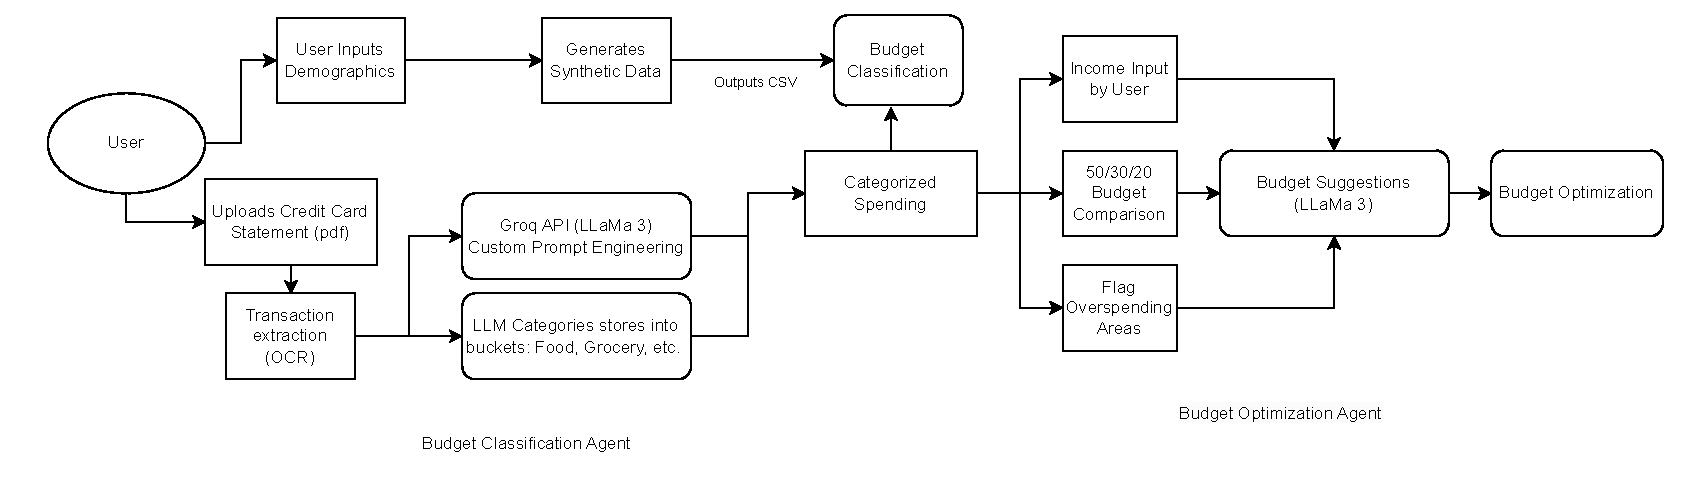
\includegraphics[width=1\linewidth]{Budget.pdf}
\caption{Budget Classification and Optimization Architecture: The user either uploads a credit card statement or provides demographic information to generate synthetic transactions. The Budget Classification Agent categorizes spending using OCR extraction and LLaMA 3-based prompt engineering. The categorized spending, along with user income, is analyzed by the Budget Optimization Agent, which applies the 50/30/20 rule and generates personalized financial recommendations using LLaMA 3.}
\label{fig:budget_flowchart}
\end{figure*}

\subsection{Classification Agent Evaluation}
We evaluated all models on a separate hold-out test set of transactions. Two metrics were used for assessment: overall Accuracy and Macro F1-score. Accuracy reflects the percentage of transactions correctly classified, while Macro F1 measures the average F1-score across all categories, giving equal weight to each category regardless of its frequency. This makes Macro F1 particularly sensitive to model performance on minority classes. Table~\ref{tab:model_comparison_classification} provides a summary of the results and key observations for each model.


\begin{table*}[htbp]
  \centering
  \caption{Model Comparison for Budget Classification}
  \resizebox{\textwidth}{!}{
  \begin{tabular}{|l|c|c|p{9cm}|}
    \hline
    \textbf{Model} & \textbf{Accuracy} & \textbf{Macro F1} & \textbf{Notes} \\
    \hline
    Logistic Regression   & $\sim$71\%           & 0.57            & Struggled with edge cases (underrepresented categories) \\
    \hline
    LSTM (RNN)            & $\sim$39\%           & 0.40            & Overfit the training data; poor generalization \\
    \hline
    BERT (Fine-tuned)     & $\sim$71\%           & 0.62            & Balanced performance, improved recall for minority classes \\
    \hline
    LLaMA-3 (Few-shot API)& \textit{N/A}         & \textit{N/A}    & High accuracy observed qualitatively (human eval); no training needed \\
    \hline
  \end{tabular}
  }
  \label{tab:model_comparison_classification}
\end{table*}


The logistic regression model achieved approximately 71\% accuracy. It performed reasonably well on frequent categories but struggled with less common classes such as “Travel” and “Education,” often due to the lack of distinctive keywords associated with those categories (for example, a travel agency name that does not explicitly reference travel may be misclassified). In contrast, the LSTM exhibited notably lower performance, with accuracy falling below 40\%. This suggests that the LSTM did not outperform the simpler logistic regression model. We attribute this to the limited size of the training dataset and the inherent noisiness of merchant names; while the LSTM may have memorized certain character sequences, it failed to generalize effectively to unseen examples.

The fine-tuned BERT model matched logistic regression in terms of overall accuracy (around 71\%) but achieved a higher Macro F1-score (0.62 compared to 0.57), indicating superior handling of underrepresented classes. BERT’s deep language understanding likely enabled it to capture subtle contextual cues and recognize synonyms, leading to improved recall for categories that are often confused—such as distinguishing between “Grocery” and “Restaurant” transactions.


Finally, the LLaMA-3 API model was not evaluated using standard metrics, as it generates predictions on demand and we were unable to conduct thousands of queries necessary for a systematic evaluation. Instead, we manually reviewed a sample of 100 randomly selected transactions classified by the LLM. The model exhibited high agreement with expected categories and showed notable adaptability to unusual cases—for example, accurately classifying a transaction from a niche local business, likely leveraging its broad pre-trained knowledge base.
Although the zero-shot model required careful prompt engineering, once properly configured, it provided a fast and flexible classification solution without consuming any labeled training data. This highlights an important trade-off between approaches: while a fine-tuned local model like BERT offers greater control and privacy, a powerful few-shot model like LLaMA-3 enables rapid deployment and flexibility. In practice, the choice between the two may depend on the application's privacy constraints and development speed requirements.


To illustrate the output of the classification agent, we integrated it into a simple user interface that aggregates categorized transactions, allowing users to see how much they spend in each category. Table~\ref{tab:spending_breakdown} shows a sample breakdown of a user’s monthly expenditures, generated from either synthetic or anonymized real transaction data. In this example, the user's spending is distributed across areas such as Travel, Grocery, Shopping, Food, and Services.

The breakdown clearly shows that \textbf{Travel} accounts for the largest share of spending, followed by \textbf{Shopping}. Other categories like \textbf{Food}, \textbf{Services}, and \textbf{Grocery} make up smaller portions. This summary enables users to quickly understand where their money is going, providing an intuitive overview of financial activity. In our system, this categorized output serves as input to the next module—the Budget Optimization Agent—which analyzes the spending pattern against budgeting guidelines and identifies opportunities for improvement.

\begin{table}[H]
\centering
\caption{Classified Spending Breakdown (Example User)}
\begin{tabular}{|l|r|}
\hline
\textbf{Category} & \textbf{Monthly Spending (\$)} \\
\hline
Travel & 181.44 \\
Shopping & 105.93 \\
Food & 51.75 \\
Services & 31.93 \\
Grocery & 26.23 \\
\hline
\end{tabular}
\label{tab:spending_breakdown}
\end{table}


\subsection{Budget Optimization Agent Design}
After the user’s spending has been categorized, the next step is to assess whether it aligns with established budgeting principles and, if not, to identify areas for potential adjustment. We use the well-known \textbf{50/30/20 rule} as our guiding framework: ideally, 50\% of post-tax income should be allocated to “needs” (essential expenses such as housing, groceries, utilities, and necessary transportation), 30\% to “wants” (discretionary spending like entertainment, dining, travel, and non-essential shopping), and 20\% to savings or debt repayment.

The Budget Optimization Agent evaluates the user’s categorized spending against these recommended proportions. To do this, each spending category is first mapped to one of the three budget buckets—needs, wants, or savings. Some categories are straightforward to classify (e.g., Grocery and Rent fall under needs, while Travel and Dining are considered wants). Savings is typically not directly observable in transaction data, but it may be inferred from transfers to savings or investment accounts, or recorded debt payments. In our implementation, we primarily focused on evaluating and adjusting essential and discretionary spending, as savings can often be estimated once those two components are accounted for.

\begin{table}[htbp]
\centering
\caption{Mapping of Spending Categories to Budget Buckets}
\label{tab:category_bucket_mapping}
\renewcommand{\arraystretch}{1.3}
\begin{tabular}{|l|l|}
\hline
\textbf{Category} & \textbf{Budget Bucket} \\
\hline
Grocery & Needs \\
\hline
Rent & Needs \\
\hline
Utilities & Needs \\
\hline
Dining & Wants \\
\hline
Entertainment & Wants \\
\hline
Travel & Wants \\
\hline
Shopping & Wants \\
\hline
Savings Transfer & Savings \\
\hline
Debt Payment & Savings \\
\hline
\end{tabular}
\end{table}


The agent identifies spending categories where the user exceeds the recommended budget thresholds. For example, with a monthly take-home income of \$2{,}000, the recommended allocation for “wants” is approximately \$600. If the combined total across discretionary categories—such as Travel, Entertainment, Dining, and Shopping—significantly surpasses that amount, the agent flags the highest contributors within this group as potential areas for reduction. Similarly, if essential spending exceeds roughly \$1{,}000 (50\% of the user’s income), the agent examines components like groceries or utilities to evaluate whether any cost savings are possible.

The agent applies this heuristic with flexibility, taking into account the user’s specific financial context. For instance, users with limited income may naturally allocate 70\% or more toward essential needs. In such cases, the agent does not rigidly enforce the 50\% threshold but instead offers suggestions for reducing necessary expenses where feasible.


\begin{table}[htbp]
\centering
\caption{Sample Budget Allocation vs.\ Actual Spending (Monthly Income = \$2{,}000)}
\label{tab:budget_allocation}
\renewcommand{\arraystretch}{1.3}
\begin{tabular}{|l|c|c|}
\hline
\textbf{Bucket} & \textbf{Target (\%)} & \textbf{Target (\$)} \\
\hline
Needs & 50 & 1{,}000 \\
\hline
Wants & 30 & 600 \\
\hline
Savings & 20 & 400 \\
\hline
\end{tabular}
\end{table}

What makes our Budget Optimization Agent interactive is its implementation as an \textbf{LLM-powered chatbot}. After receiving the categorized spending data and the user’s income from the classification agent, the optimization module generates a natural language response. To do so, we prompt an LLM (specifically, the Groq LLaMA-based model or an equivalent GPT-3.5-class model) with key user details, including income, per-category spending, and any categories where spending exceeds recommended targets. 
The structure of the prompt is designed to encourage detailed, personalized suggestions. An example prompt is shown below:

\begin{quote}
\small
\texttt{
Based on the user's demographics and spending, provide personalized budget optimization suggestions.\\
- In grocery recommendations, include different store names based on affordability and general popularity.\\
- Suggest specific action steps for groceries, shopping, travel, and other overspending areas. Estimate potential monthly savings based on the user's profile.\\
- Adjust advice based on the user's income levels}
\end{quote}
The LLM then generates a conversational output, which is presented to the user. These responses include actionable recommendations, phrased in a supportive, coaching tone to encourage engagement and financial improvement.



\subsection{Optimization Advice and Interface}
The advice generated by the agent is based on the user's individual spending patterns. For example, if \textbf{Groceries} are identified as an area of high spending, the agent might suggest practical strategies such as shopping at discount stores, buying in bulk, or meal planning to reduce waste. If \textbf{Services} (such as recurring subscriptions or utility bills) are flagged as excessive, the agent may recommend canceling unused subscriptions or negotiating lower rates for phone or internet services. Using an LLM allows the system to produce more specific and actionable advice, rather than offering simple rules like "cut 10\% from groceries." The agent can also acknowledge that some expenses are necessary and encourage users to find savings where possible.

We developed a simple chat-style interface where users can view the agent’s recommendations and optionally ask follow-up questions. In our prototype, after the initial suggestions are displayed, the user can request additional ideas or clarification (for example, “What other ways can I save on groceries?”), and the LLM will generate a response accordingly, supporting a more interactive budgeting experience.

To evaluate this component, we constructed a test scenario. \textbf{Scenario:} A user with an annual income of \$24,500 (approximately \$2{,}042 per month) was simulated with the following monthly expenditures: Food (restaurants) at \$200, Groceries at \$500, Travel at \$300, Services (e.g., phone, internet, subscriptions) at \$450, and Shopping at \$250, with other minor categories making up the remainder. Overall, essential expenses—covering Groceries, a portion of Services, and essential Shopping—totaled approximately \$1,200, exceeding the recommended \$1,021 target for needs (50\% of income). Discretionary spending—including Travel, non-essential Services, and discretionary Shopping—was around \$800, which also surpassed the \$612 guideline for wants (30\% of income).

The agent identified \textbf{Grocery} and \textbf{Services} as the categories where spending was most above the recommended limits. It then focused its advice on these areas. For groceries, the agent suggested shopping at discount supermarkets, mentioning examples such as Aldi and Lidl, and recommended meal planning as a strategy to reduce unnecessary purchases. For services, it advised reviewing subscriptions to cancel any that were no longer needed and considering lower-cost alternatives, such as switching to a more affordable phone plan or bundling internet and phone services for potential savings.
The agent also provided an estimate of the possible financial impact: by following the suggestions, the user could save approximately \$70 to \$100 per month. In this scenario, the potential savings were broken down into about \$50 from groceries and \$20 to \$30 from services, corresponding to an overall budget improvement of approximately 3--5\%.



\begin{table*}[htbp]
  \centering
  \caption{Budget Optimization Recommendations (Example Scenario)}
  \resizebox{\textwidth}{!}{
  \begin{tabular}{|l|p{6cm}|p{7cm}|c|}
    \hline
    \textbf{Category} & \textbf{Issue} & \textbf{Recommendation} & \textbf{Estimated Monthly Savings} \\
    \hline
    Grocery  & Spending above essential budget & Shop at discount supermarkets; plan meals and buy in bulk to reduce costs. & \$50 (approx) \\
    \hline
    Services & Multiple subscriptions (high total) & Cancel or downgrade unnecessary subscriptions; negotiate lower rates for utilities/internet. & \$30 (approx) \\
    \hline
  \end{tabular}
  }
  \label{tab:budget_optimization_recommendations}
\end{table*}


In Table~\ref{tab:budget_optimization_recommendations}, we summarize the main recommendations for the two categories identified in the example scenario. These suggestions were generated by the LLM, and the estimated savings were based on reasonable assumptions (for example, switching to lower-cost grocery stores was estimated to save approximately \$50 per month, while reducing service-related expenses could save about \$30). In the user interface, the optimization agent combined these recommendations into a conversational message. An example chatbot output is shown below:

\begin{quote}
\textit{“It looks like your \textbf{grocery spending} is a bit high. You might try switching to discount supermarkets like Aldi or Lidl, and make a meal plan each week – this can save quite a bit! Also, your \textbf{services and subscriptions} are higher than typical. Consider canceling any subscriptions you don’t use regularly (streaming services, gyms, etc.), or see if you can find a better phone plan or bundle to lower those bills. Together, these changes could save you around \$80 a month, which you could put towards savings or other needs.”}
\end{quote}

We found this approach effective for providing specific and practical advice. A small user study involving a few volunteers (using either their own financial data or synthetic profiles) showed that participants found the suggestions useful and concrete, rather than vague or overly general. Users appreciated receiving clear, actionable tips instead of broad advice like “spend less on entertainment.”

One ongoing challenge is ensuring the accuracy and reliability of the financial advice produced by the LLM. In our prototype, we manually reviewed the suggestions to verify they were reasonable. However, future improvements could include implementing an automated review step or fine-tuning the LLM on datasets specific to personal finance, in order to reduce the risk of inappropriate or inaccurate advice. Overall, the Budget Optimization Agent shows how combining structured budgeting rules (like the 50/30/20 guideline) with conversational AI can provide users with practical ways to manage and improve their finances.

After developing a personalized spending plan through the Budget Optimization Agent, the next logical step toward improving financial well-being is determining how to put the saved income to effective use. In many situations, optimizing expenses can free up hundreds or even thousands of dollars that can be redirected from discretionary spending into activities that support long-term financial growth. Recognizing this opportunity, we extended the system to include an investment advisory component. 

The motivation is straightforward: financial planning does not stop with saving; it must also address how to invest savings wisely. With a portion of the user's budget now available for potential investment, our system moves to the third major component: the \textbf{LLM-Advisor}. This module is designed to provide intelligent, data-driven, and explainable investment suggestions, incorporating both real-time market information and user-specific profiles. While the earlier modules focused on promoting financial efficiency and spending discipline, this next phase aims to build on those improvements by helping users grow their capital through AI-assisted investment guidance.


\section{LLM-Advisor: Personalized Investment Advisory System}

The third part of our platform is an AI-driven investment consultant, referred to as \textbf{LLM-Advisor}, designed to deliver tailored investment advice. This component considers \textit{real-time financial data} (market prices, news updates, and company fundamentals) along with the {user’s profile} to recommend a portfolio or specific trading actions (e.g., buy, sell, or hold particular stocks or assets). What sets our advisor apart from conventional quantitative trading systems is the fusion of \textbf{LLM models)} with explanation generation—it not only processes numerical signals but also ``reads'' the news, gauges market sentiment, and can articulate its reasoning in plain English. The LLM-Advisor’s architecture comprises several modules working together:

\subsection{Data Ingestion and Processing}

The advisor requires timely market and asset information to inform its recommendations. To achieve this, we built a data retrieval layer using the \texttt{yfinance} API (a Python interface to Yahoo Finance) to fetch both real-time quotes and historical records. For each security, the system collects the latest price metrics (e.g., daily closing prices), pertinent \textbf{news headlines}, and essential \textbf{fundamental data}—including financial statements and ratios such as price-to-earnings, market capitalization, and recent earnings releases. For example, when advising on Apple Inc., the advisor gathers Apple’s price history, recent news coverage, and its latest quarterly earnings report. This ingestion process runs on a set schedule or on-demand whenever the user requests guidance on a specific asset or portfolio. By combining numerical price data with qualitative news insights, the advisor attains a multidimensional perspective on each asset. In this project, we have initialized our analysis universe with a curated list of 20 stocks, organized into aggressive (high-risk), balanced (medium-risk), and conservative (low-risk) profiles.

\subsection{Ensemble Sentiment Analysis}

A key capability of our LLM-Advisor is its ability to analyze the \textit{sentiment} of news and media, thereby capturing the market’s prevailing mood toward an investment. To achieve this, we utilize an \textbf{ensemble of three sentiment analysis models} for financial news evaluation: (1) \textbf{FinBERT}, a BERT-based model pre-trained on financial texts and fine-tuned specifically for sentiment classification in the financial sector~\cite{b3}; (2) \textbf{RoBERTa}, a leading transformer architecture fine-tuned on a finance-related sentiment dataset to offer broader language understanding~\cite{b4}; and (3) \textbf{VADER} (Valence Aware Dictionary and sEntiment Reasoner), a lexicon- and rule-based tool optimized for short-form content such as social media posts~\cite{b5}.

Each news headline or snippet is processed by all three models. FinBERT, with its financial focus, assigns labels of Positive, Neutral, or Negative. RoBERTa follows the same classification, while VADER outputs a compound sentiment score between $-1$ (very negative) and $+1$ (very positive). We then map VADER’s continuous score to a discrete Positive/Neutral/Negative label using standard thresholds (e.g., score $>0.05$ = Positive, score $< -0.05$ = Negative).

The ensemble merges these results -- aggregating votes or averaging confidence scores from FinBERT and RoBERTa, with VADER’s output serving as a tiebreaker or supplementary signal. When all three models align (for example, all indicate positive sentiment), our confidence is high. If their assessments differ, we use a majority vote or assign greater weight to FinBERT for finance-specific content, while RoBERTa captures nuances that FinBERT might miss (such as sarcasm or unconventional phrasing), and VADER helps detect subtle negativity (or positivity) in brief, social media–style texts.

The ensemble’s output is a sentiment indicator for the asset, typically expressed as: ``Overall news sentiment for \textit{Stock X} this week is \textbf{Positive}'' or presented as a numerical score. This sentiment feed is essential—numerous studies and trading strategies treat sentiment as a leading signal for short-term market movements (for example, a wave of negative headlines can drive a stock downward before any fundamental changes occur).


\begin{figure}[htbp]
\centering
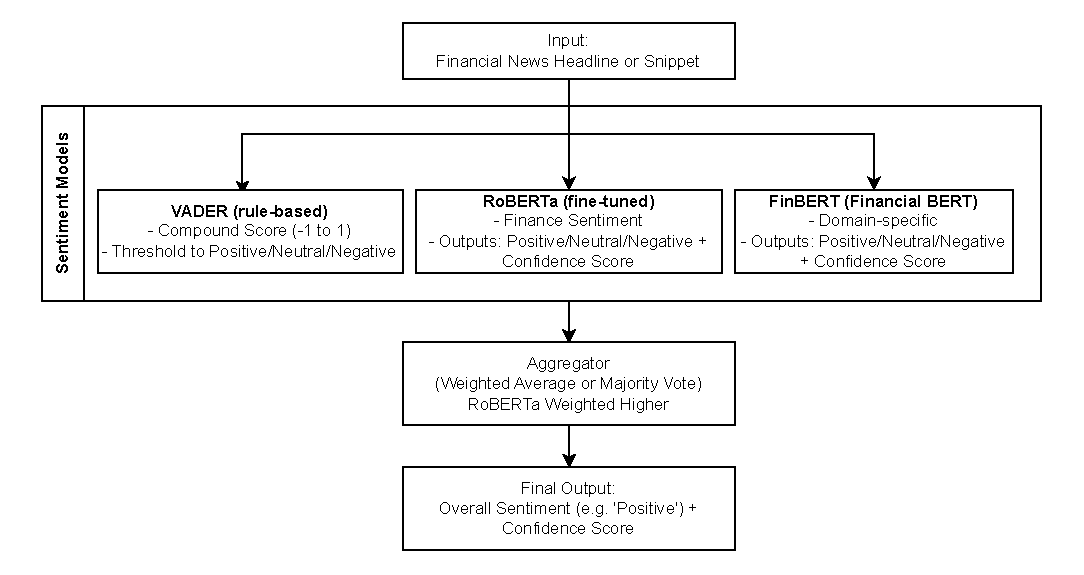
\includegraphics[width=\linewidth]{Ensemble.pdf}
\caption{Architecture of the Ensemble Sentiment Analysis Model combining FinBERT, RoBERTa, and VADER outputs using a weighted aggregation strategy. This ensemble produces a final overall sentiment classification along with a confidence score, enhancing reliability by leveraging domain-specific and general language models.}
\label{fig:ensemble_architecture}
\end{figure}

As an illustrative output of this module, we present a sample sentiment analysis breakdown for Tesla-related headlines, processed by our ensemble of FinBERT, RoBERTa, and VADER. This example shows how the advisor transforms raw news into actionable insights:

\begin{table*}[htbp]
\renewcommand{\arraystretch}{1.3} % Increases row height
\centering
\caption{Example Sentiment Analysis Output: Tesla News Headlines Evaluated by the Ensemble Model.}
\label{tab:tesla_sentiment}
\begin{tabular}{|p{10cm}|c|c|}
\hline
\textbf{Headline} & \textbf{Score} & \textbf{Sentiment} \\
\hline
Tesla's fight for survival: Why Americans are abandoning the brand and Elon Musk & -0.63 & Negative \\
\hline
Donald Trump shares thoughts on Elon Musk's DOGE step back & 0.06 & Neutral \\
\hline
JPMorgan Chase \& Co. has lowered expectations for Tesla stock price & -0.53 & Negative \\
\hline
Robert W. Baird cuts Tesla stock price target to \$395 & -0.06 & Neutral \\
\hline
\end{tabular}
\end{table*}

This table underscores the advisor’s ability to synthesize multiple NLP tools into a consistent and explainable sentiment signal. The ensemble approach helps avoid false positives or negatives that any single model might produce (see Table~\ref{tab:tesla_sentiment}).

To further demonstrate how different sentiment models contribute to the final ensemble decision, we show a side-by-side comparison of sentiment labels assigned by FinBERT, RoBERTa, and the Ensemble model for the same set of financial headlines. This comparison (Table~\ref{tab:sentiment_model_comparison}) highlights how the models occasionally disagree and how the ensemble offers a balanced, often more accurate, final interpretation.


\begin{table*}[htbp]
\renewcommand{\arraystretch}{1.3}
\centering
\caption{Comparison of Sentiment Labels Across Models for Sample Financial News Headlines}
\label{tab:sentiment_model_comparison}
\begin{tabular}{|p{8cm}|p{2.5cm}|p{2.5cm}|p{2.5cm}|}
\hline
\textbf{News Headline} & \textbf{FinBERT Label} & \textbf{RoBERTa Label} & \textbf{Ensemble Label} \\
\hline
Apple beats earnings expectations, iPhone sales rebound & Positive & Positive & \textbf{Positive} \\
\hline
Ford warns of EV margin pressures in upcoming quarter & Negative & Neutral & \textbf{Negative} \\
\hline
Amazon expands grocery delivery across U.S. cities & Neutral & Positive & \textbf{Positive} \\
\hline
Netflix faces subscriber loss after price hikes & Negative & Negative & \textbf{Negative} \\
\hline
Google’s AI division sees modest growth amid tough competition & Neutral & Neutral & \textbf{Neutral} \\
\hline
\end{tabular}
\end{table*}


This example illustrates several key takeaways: while FinBERT often picks up clear sentiment in financial context, RoBERTa sometimes softens or reinterprets tone due to its general domain nature. The ensemble aggregates these perspectives, sometimes overriding individual predictions when the overall sentiment is clearer. For instance, in the Amazon headline, FinBERT failed to catch the positive expansion signal, while RoBERTa did—leading the ensemble to correctly mark it as \textbf{Positive}.


\subsection{Fundamental Analysis Module}

Alongside sentiment analysis, the advisor examines \textbf{fundamental indicators} for each asset~\cite{yfinance2023}. Using data pulled via \texttt{yfinance}~\cite{yfinance2023}, it calculates or extracts metrics like revenue growth, profit margins, debt-to-equity ratio, and sector-relative P/E ratio. Rather than employing a black-box model, we implemented a clear rule-based assessment combined with an LLM-generated summary~\cite{finbert2020}. For instance, the system might ask: is the company’s revenue rising year-over-year? Does its P/E ratio diverge notably from the industry average? Is its debt level sustainable? These criteria are aggregated into a fundamental score or expressed as descriptive summaries (e.g., ``Company A has strong fundamentals with consistent growth and low debt'' or ``Company B’s fundamentals are weak: declining sales and high valuation multiples''). We further allow the LLM to parse qualitative sections of financial reports (such as the management’s discussion and analysis) to capture nuanced insights~\cite{bloomberggpt2023}, though our current approach emphasizes numeric factors. These metrics can feed into a simple model or be applied directly in decision logic. Consequently, a stock with solid fundamentals (robust growth, undervaluation relative to peers) will generally lead the advisor to suggest a \textbf{Buy}, barring any overriding considerations.


\subsection{Technical Analysis Module}

In addition to long-term fundamentals and short-term sentiment, we include \textbf{technical indicators} to gauge market timing~\cite{hossain2019}. The technical module computes indicators like \textbf{Relative Strength Index (RSI)}, \textbf{Moving Average Convergence Divergence (MACD)}, and simple moving averages (50-day and 200-day) from price data. These are well-known indicators among traders: RSI indicates whether a stock is overbought or oversold (typically, RSI > 70 means overbought, < 30 oversold), MACD signals trend changes when its signal line crosses, and moving average crossovers (e.g., the 50-day moving above the 200-day, the so-called ``golden cross'') can indicate momentum shifts~\cite{hossain2019}. We use a set of such rules to form a \textbf{technical score}. For example, we add +1 to the score if the stock’s price is above its 50-day average (an indicator of recent strength), +1 if the 50-day average is above the 200-day (indicating an uptrend), +1 if RSI has recently risen above 60 (signaling bullish momentum coming out of an oversold condition), and similarly subtract points for bearish signals (RSI dropping below 40, price below moving averages, etc.). This yields a net technical score that might range from, say, –4 to +4. We then normalize this to a confidence factor between 0 and 1. The idea is that even if fundamentals and sentiment are good, if technical indicators are currently very bearish, the advisor might caution the user or suggest waiting for a better entry point. Conversely, if technicals align positively with good news, the advisor will have stronger conviction in a recommending that stock. 

Beyond assessing long-term fundamentals and short-term sentiment, our advisor also incorporates \textbf{technical indicators} to refine market timing. The technical analysis module calculates measures such as the \textbf{Relative Strength Index (RSI)}, \textbf{Moving Average Convergence Divergence (MACD)}, and simple moving averages (50-day and 200-day) from price data~\cite{hossain2019}. These are standard tools for traders: RSI highlights overbought (RSI > 70) or oversold (RSI < 30) conditions; MACD signals trend reversals when its signal line crosses the MACD line; and moving average crossovers (for example, the 50-day average rising above the 200-day, known as a “golden cross”) indicate momentum shifts. We translate these rules into a \textbf{technical score}. For example, we assign +1 if the stock’s price is above its 50-day average (signaling recent strength), +1 if the 50-day average exceeds the 200-day (indicating an uptrend), +1 if RSI recently climbed above 60 (marking emerging bullish momentum), and subtract points for bearish signals (e.g., RSI falling below 40 or price dipping below moving averages). This yields a raw technical score typically ranging from –4 to +4, which we then normalize to a 0–1 confidence factor. As a result, even when fundamentals and sentiment appear favorable, strongly negative technicals may lead the advisor to suggest waiting for a better entry. Conversely, when technicals align with positive news, the system gains higher confidence in a \textbf{Buy} recommendation.
 


\begin{figure*}[htbp]
\centering
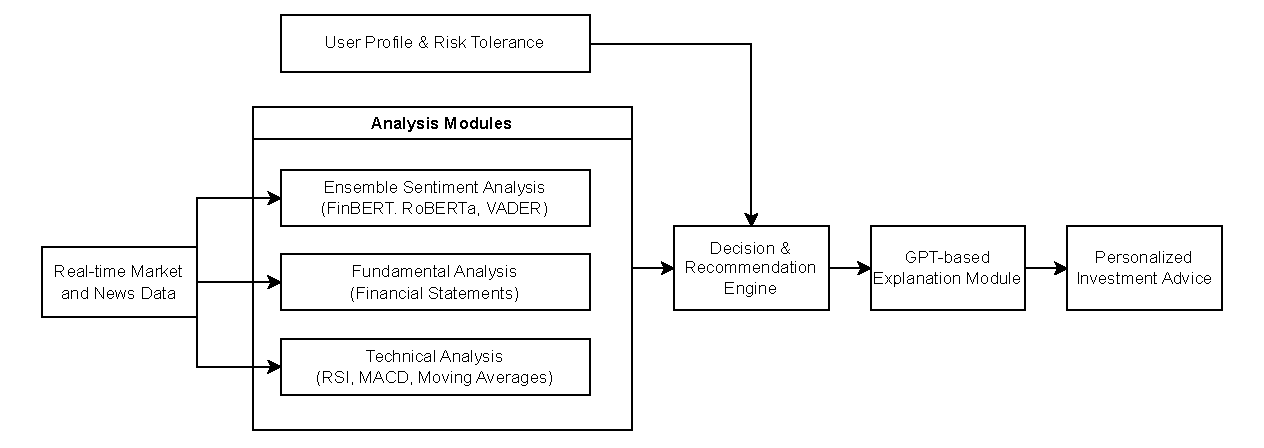
\includegraphics[width=0.8\textwidth]{Investment.pdf} % <-- scaled down to 75% of text width
\caption{LLM-Advisor Architecture.}
\label{fig:llm-advisor-architecture}
\end{figure*}



The investment advisor agent comprises several analytical modules that draw on diverse data sources. It begins by retrieving real-time market data and news for the selected assets, alongside the user’s profile information (including risk tolerance). The system executes an \textbf{ensemble sentiment analysis} on news headlines (via FinBERT~\cite{b3}, RoBERTa~\cite{b4}, and VADER~\cite{b5}) to capture market mood. Concurrently, it performs \textbf{fundamental analysis} by extracting and evaluating financial statements and key ratios, and \textbf{technical analysis} by calculating indicators such as RSI, MACD, and moving averages from price histories~\cite{hossain2019}. These insights converge in a central \textbf{Decision \& Recommendation Engine}, which combines the signals—a robust positive sentiment and strong fundamentals might trigger a ``Buy'' recommendation, moderated by technical trends and tailored to the user’s risk profile. The user’s risk tolerance then refines the output (for example, favoring higher-volatility selections for aggressive profiles and safer assets for conservative ones). Finally, a \textbf{GPT-based Explanation Module} transforms the decision logic into clear natural language, delivering both the recommendation and its rationale to the user. This design enables the advisor to synthesize structured and unstructured inputs and offer actionable guidance alongside understandable explanations.



\subsection{Risk Profiling and Recommendation Generation}

A cornerstone of effective investment advice is tailoring it to the \textbf{user’s risk profile}. Investors are typically grouped—via a questionnaire or known preferences—into \textit{Conservative}, \textit{Moderate}, or \textit{Aggressive} categories. Our advisor reflects this by adjusting both the recommendation style and allocation sizes.

The agent offers recommendation in two formats:

\begin{enumerate}
    \item \textbf{Single Stock Recommendation:} When a user asks about a specific stock (e.g., ``What do you think of Apple?''), the agent replies with its recommendation accompanied by a confidence score. This score combines the model’s output probability with the consensus among technical, sentiment, and fundamental analyses. For instance, if FinBERT~\cite{b3} forecasts a 75\% chance of an upward move, technical indicators are bullish~\cite{hossain2019}, and sentiment is positive, the agent might favorably recommend the stock. If signals conflict (e.g., bullish model output but weak fundamentals), the recommendation could be softened to ``Hold''.
    
    \item \textbf{Portfolio Recommendation:} If the user requests a portfolio or specifies a risk level, the agent constructs an example portfolio aligned with one of three profiles: Low, Medium, or High risk.
    
    \begin{itemize}
        \item \textbf{Low Risk:} Focus on large-cap, stable companies with dependable dividends or defensive sectors (e.g., consumer staples, healthcare)~\cite{alobaidi2022}, ensuring none exhibit strongly negative sentiment or technical signals.
        \item \textbf{Medium Risk:} A balanced mix of stable and growth-oriented stocks, often including blue-chip tech names.
        \item \textbf{High Risk:} Higher-volatility or high-upside picks, such as tech startups, companies riding strong sentiment or technical momentum, and speculative assets.
    \end{itemize}
    
    Allocation follows simple heuristics: in a low-risk portfolio, the two safest stocks might each receive 30--40\% of the weight, with 10--15\% spread among others for diversification. High-risk portfolios may either spread weights more evenly or concentrate them on top convictions, always summing to 100\%.
\end{enumerate}

Illustrative outputs include:
\begin{quote}
\textit{Low-Risk Portfolio:} 40\% in JNJ (Johnson \& Johnson), 30\% in KO (Coca-Cola), 20\% in WMT (Walmart), 10\% in MSFT (Microsoft). These selections offer defensive stability and strong fundamentals.
\end{quote}
\begin{quote}
\textit{High-Risk Portfolio:} 25\% in TSLA (Tesla), 20\% in NVDA (Nvidia), 20\% in COIN (Coinbase), 20\% in GME (GameStop), 15\% in AMD. These picks carry higher volatility and growth potential but come with greater risk.
\end{quote}

To demonstrate a real instance of portfolio construction by our agent, we present a medium-risk portfolio sample below. The stocks are selected based on the ensemble signals, confidence scores, and price allocation strategy.


\begin{table*}[htbp]
\renewcommand{\arraystretch}{1.3} % Increases row height
\centering
\caption{Medium-Risk Portfolio Generated by LLM-Advisor. Portfolio allocation is based on confidence score, price, and diversification strategy for a \$2,344 investment.}
\label{tab:medium_portfolio}
\begin{tabular}{|l|l|l|c|c|c|c|}
\hline
\textbf{Stock} & \textbf{Sector} & \textbf{Trend} & \textbf{Confidence} & \textbf{Price} & \textbf{Shares} & \textbf{Allocation} \\
\hline
AAPL & Tech   & UP & 88.9\% & \$200.01 & 3 & \$788.29 (33.6\%) \\
\hline
F    & Auto   & UP & 88.3\% & \$9.66   & 81 & \$783.24 (33.4\%) \\
\hline
HD   & Retail & UP & 87.1\% & \$354.15 & 2 & \$772.46 (33\%) \\
\hline
\end{tabular}
\end{table*}


\vspace{0.5em}
This portfolio reflects the agent’s balance between sectors and stock-specific confidence. Such breakdowns can be directly communicated to users, enabling clear decision-making aligned with their investment profile~\cite{lakkaraju2023}.

\vspace{0.5em}

To make the final decision, the agent applies the following rule-based thresholds derived through trial and error and validated on a small development set~\cite{hossain2019}:
\begin{itemize}
    \item If probability of Up $>0.7$ and at least two of the other three signals (technical, sentiment, fundamental) are positive, then \texttt{recommendation = "Buy (High confidence)"}.
    \item If probability of Up is moderate (0.4--0.7) and signals are mixed, \texttt{recommendation = "Hold/Neutral"}.
    \item If probability of Up is low $<0.3$ or multiple negative signals, \texttt{recommendation = "Sell"}.
\end{itemize}

The core analyses—sentiment, fundamentals, and technicals—are applied uniformly across all risk profiles~\cite{hossain2019}. The distinction lies in how stringent the thresholds are: for a conservative profile, a ``Buy'' recommendation may only be issued when every indicator is strongly positive, whereas an aggressive profile may tolerate greater risk and act on partial signals.

\vspace{0.5em}

All recommendations include clear disclaimers, emphasizing that these are academic suggestions and not financial advice~\cite{fieberg2023}. The agent is tailored for short- to medium-term horizons (from days up to several months), assuming an active investor will rebalance positions as market conditions evolve.



\subsection{Evaluation and Example Scenario}

We evaluated the LLM-Advisor’s performance in two ways: (1) by testing the accuracy of its individual components (e.g., sentiment classifier, predictive power of signals), and (2) through end-to-end hypothetical scenarios to see if the advice aligns with what a human financial analyst might say.

For the first part, we created a dataset of historical stock movements to measure how well our sentiment models (FinBERT, etc.) and combined signals predict actual market outcomes~\cite{finbert2020, brown2020}. We collected closing prices and technical indicators for a set of stocks over a period (e.g., 2015--2024) along with the next-day stock movement (up or down). We then fine-tuned FinBERT and also a DeBERTa-v3 model (a newer transformer model known for strong language understanding) to predict stock movement (up/down), as a proxy evaluation of our technical analysis~\cite{deepfinance2021}. \textbf{Table III} shows the performance of these models under different training settings (training on 4 years vs 10 years of data, with and without oversampling the minority class to address class imbalance). This evaluation, while not directly the final advisor's output, provided insight into how informative the stock data and technical features are.

\vspace{0.5em}

We assessed the LLM-Advisor’s performance using two strategies: (1) evaluating the accuracy of its individual modules (e.g., the sentiment classifier and the predictive power of our signals), and (2) running end-to-end hypothetical scenarios to verify whether its recommendations match those of a human financial analyst.

For the first strategy, we assembled a historical stock movement dataset to gauge how well our sentiment models (such as FinBERT) and combined indicators anticipate real market shifts~\cite{finbert2020, brown2020}. This dataset comprised daily closing prices and technical metrics for selected stocks over the period 2015--2024, along with labels indicating the direction of the next day (up or down). We fine-tuned both FinBERT and DeBERTa-v3—a more recent transformer noted for strong language understanding—to predict these up/down movements as a proxy for evaluating our technical analysis~\cite{deepfinance2021}. \textbf{Table III} displays the performance of the models in different training scenarios (four years versus ten years of data, with and without oversampling the minority class to address the class imbalance). Although this evaluation does not directly reflect the advisor’s final recommendations, it offers insight into the informativeness of our price data and technical features.


\begin{table*}[htbp]
\centering
\small % Reduce font size
\renewcommand{\arraystretch}{1.3} % Increase row height for clarity
\caption{Stock Movement Prediction Model Performance. \textit{(FinBERT and DeBERTa models fine-tuned to predict next-day stock price movement from technical indicators; evaluated on approx. 48,000 data samples from the last 10 years.)}}
\label{tab:stock-movement-prediction-model-performance}
\begin{tabular}{|l|c|c|c|c|}
\hline
\textbf{Model (Training Data)} & \textbf{Accuracy} & \textbf{Precision} & \textbf{Recall} & \textbf{F1} \\
\hline
FinBERT (4-year, no oversample)    & 0.525 & 0.537 & 0.511 & 0.523 \\
FinBERT (10-year, no oversample)   & 0.561 & 0.567 & 0.590 & 0.633 \\
FinBERT (10-year, with oversample) & 0.535 & 0.602 & 0.628 & 0.615 \\
DeBERTa (4-year, no oversample)    & 0.518 & 0.541 & 0.503 & 0.536 \\
DeBERTa (10-year, no oversample)   & 0.538 & 0.670 & 0.640 & 0.655 \\
DeBERTa (10-year, with oversample) & 0.569 & 0.651 & 0.680 & 0.685 \\
\hline
\end{tabular}
\end{table*}



From Table~\ref{tab:stock-movement-prediction-model-performance}, we note several patterns. Models trained on a 10-year dataset outperformed those trained on only 4 years—DeBERTa’s accuracy, for example, rose from approximately 52\% to about 57\% when using more data~\cite{brown2020}. Applying oversampling to the minority class (e.g., fewer “up” days than “down” days) tended to boost Recall (detecting “up” movements) while slightly reducing Precision, reflecting a typical trade-off~\cite{deepfinance2021}. The top performer was DeBERTa trained on 10-year data with oversampling, reaching an F1-score around 68.5\%. Although these metrics only modestly exceed random chance (50\% accuracy, F1=0.5 for random guessing), they demonstrate that the dataset contains a useful predictive signal. Comparing FinBERT and DeBERTa revealed that, with sufficient data, the more general DeBERTa model edged out the finance-specific FinBERT~\cite{finbert2020}, indicating its advanced architecture can effectively learn this domain even without inherent financial pre-training. Nevertheless, FinBERT remained competitive, particularly on the smaller (4-year) dataset, likely benefiting from its specialized in-domain knowledge in data-scarce scenarios.

\subsection{Model Training and Backtesting for Stock Prediction}

To assess the investment agent’s predictive performance, we applied a backtesting procedure to our fine-tuned FinBERT model~\cite{finbert2020}. We reframed the stock movement task as a binary classification: given recent stock characteristics, predict whether the price will move \emph{Up} or \emph{Down} on the next trading day.

Instead of using raw numerical inputs, we leveraged FinBERT’s natural language capabilities by converting technical indicators into text-based prompts. For example: \textit{“Price up 2\% today, trading above the 20-day moving average, RSI=60, low volatility — next-day move?”}. Each prompt was labeled according to the actual direction on the following day.

We created the training set from historical price data of our 20-stock universe spanning February 1, 2025 to April 15, 2025. For each stock on each date, we calculated technical features, formatted them as prompts, and assigned the subsequent day’s movement (\emph{Up}/\emph{Down}) as the label. This dataset was then used to fine-tune the FinBERT model from the ProsusAI checkpoint.

After training and choosing the best checkpoint based on a validation split, we conducted a backtest over a held-out period (late March through mid-April 2025). During this phase, the model issued daily predictions for each stock, which we compared against the actual outcomes.

\begin{table}[ht]
\centering
\caption{Backtesting performance of the fine-tuned FinBERT model on stock movement prediction (Up/Down daily).}
\label{tab:backtest}
\begin{tabular}{lc}
\hline
\textbf{Metric} & \textbf{Score} \\
\hline
Accuracy & 0.60 \\
Precision (Up) & 0.58 \\
Recall (Up) & 0.62 \\
F$_1$-score (Up) & 0.60 \\
\hline
\end{tabular}
\end{table}
These findings suggest that, despite the inherent difficulty of predicting short-term stock movements, our model successfully uncovers actionable patterns from the textual technical prompts. Achieving roughly 60\% accuracy—versus a 50\% random baseline—indicates that fine-tuning FinBERT on structured language inputs yields predictive signals that reinforce the advisor’s recommendations~\cite{finbert2020}.

Although the advisor’s ensemble sentiment component does not directly produce a binary up/down forecast as shown in Table~\ref{tab:stock-movement-prediction-model-performance}, this backtesting exercise confirmed that our sentiment pipeline is effective and contributory~\cite{deepfinance2021}. In the final system, sentiment signals are weighed alongside fundamental and technical analyses before issuing any recommendation.

\subsection{Holistic end-to-end Scenario: How the LLM-Advisor Could Assist an Investor}

To demonstrate the LLM-Advisor in action, consider a hypothetical \textit{Moderate risk} investor evaluating two stocks: a technology firm (TechCo) and a utility provider (UtilCo). On a given day, TechCo reports strong earnings, paired with overwhelmingly positive news sentiment and solid fundamentals (e.g., high revenue growth and healthy profit margins), although its rapid price increase suggests it may be slightly overbought according to technical indicators~\cite{brown2020}.

In contrast, UtilCo shows a stable outlook: neutral sentiment, flat earnings, and a mild technical downtrend, reflecting its typically lower-risk profile.

In this scenario, the LLM-Advisor’s multi-signal analysis might yield:

\begin{itemize}
  \item \textbf{TechCo}: Recommend a \textbf{Buy}, with a caveat: \textit{"TechCo’s recent performance is impressive—news sentiment is very positive, and fundamentals are strong. However, given the short-term price spike and your moderate risk tolerance, a phased buying strategy may be prudent. TechCo could enhance growth within a diversified portfolio."}
  \item \textbf{UtilCo}: Recommend a \textbf{Hold} (or a slight position increase for stability): \textit{"UtilCo remains a dependable utility stock with consistent, though modest, fundamentals. Its small price dip may offer an opportunity to bolster your defensive holdings. For a moderate-risk investor, maintaining or marginally increasing exposure could improve portfolio resilience."}
\end{itemize}

This example highlights how the LLM-Advisor blends sentiment, fundamental, and technical insights to deliver nuanced advice aligned with risk preferences. While comprehensive conversational evaluation is pending, early prototypes and user feedback indicate the system can mirror the balanced, transparent guidance of a human analyst.

Users particularly valued the GPT-based explanations for their clarity—avoiding technical jargon (e.g., stating "price has spiked" rather than "RSI=75"). Future work will focus on formal user studies to rigorously assess the quality and clarity of these recommendations and explanations~\cite{fieberg2023}.


\subsection{System Performance and Discussion}

In terms of response time, the LLM-Advisor generates results in only a few seconds per query on our infrastructure (running FinBERT fine-tuned on a GPU and invoking the GPT module via a swift API call). Its architecture is both modular and scalable; any individual component, whether sentiment analysis, technical indicator computation, or another task can be upgraded or replaced without affecting the rest of the system. For example, if a more advanced finance-specialized language model such as BloombergGPT~\cite{b7} becomes accessible, we could integrate it into the explanation engine or even substitute it for our sentiment analysis component. BloombergGPT has outperformed general purpose models in many finance-related NLP benchmarks~\cite{b7}, suggesting that adopting such models can further enhance advisor capabilities. Furthermore, while our prototype currently targets stock recommendations, the same modular design could be applied to other domains, such as cryptocurrency, ETFs (where social media sentiment is paramount) or real estate (where news and macroeconomic indicators play a significant role).

An issue we faced was maintaining the \textbf{consistency} of the advice. Since the explanation is generated by an LLM, any imprecision in the input summary can lead the model to introduce embellishments or minor exaggerations. We addressed this by carefully designing the explanation prompt and explicitly listing the key points to include. In a production environment, we would likely adopt a templated or more constrained generation approach to ensure regulatory compliance, which is critical in finance, where irresponsible recommendations have serious implications~\cite{fieberg2023}. Another obstacle is \textbf{evaluation}: unlike simple classification metrics, evaluating the quality of investment advice is inherently subjective and often depends on long-term results. We focused on verifying that the recommendations are sensible and align with established expert practices, rather than promising guaranteed profits. For future versions, integrating a backtesting framework would allow us to simulate how the agent’s suggestions would have performed over historical periods.

To conclude, the LLM-Advisor component illustrates the potential of blending \textbf{AI-driven analytics} with \textbf{human-like advisory interaction}. It merges cutting-edge NLP techniques—transformer-based sentiment analysis and GPT-generated explanations—with traditional financial analysis methods, forming a hybrid framework~\cite{b7,bloomberggpt2023}. By delivering both actionable recommendations and clear justifications, it meets a critical need in financial services -- the need for explainable and trustworthy AI. Overall, our integrated system, spanning data generation, personal budgeting, and investment advising, demonstrates how advanced machine learning can empower individuals across all facets of personal finance.


\section{Conclusion}

We have described an end-to-end AI-driven financial intelligence platform covering three tightly linked domains: synthetic data creation, personal budgeting, and investment guidance. The \textbf{Synthetic Data Generator} addresses the scarcity of open financial transaction datasets by synthesizing realistic records. Leveraging demographic-based simulations~\cite{acsdata}, GAN-enhanced refinement~\cite{ctgan2019}, and innovative LLM-driven augmentation~\cite{brown2020}, it produces data that mirrors genuine spending patterns while safeguarding user privacy. Such synthetic datasets are invaluable for researchers and organizations to build and validate financial models without exposing sensitive information.

Leveraging either this synthetic data or actual user data, the \textbf{Budget Classification and Optimization agents} function as an automated personal finance aide. The classification agent sorts raw transaction logs into relevant categories with high precision—exceeding 70\% accuracy and achieving more balanced category distributions via a fine-tuned BERT model~\cite{b6}. Crucially, we demonstrate that LLMs can accomplish this categorization in a few-shot setting~\cite{brown2020}, offering a rapid-deployment alternative when labeled data is limited. The optimization agent then transforms these categorized insights into practical budgeting advice, grounded in proven financial principles~\cite{b8}. Through an LLM-powered conversational interface, it delivers customized recommendations—such as switching to more economical retailers or cancelling underused subscriptions—that can generate substantial monthly savings, illustrating the system’s real-world benefits at scale.

Finally, the \textbf{LLM-Advisor} represents a major step forward in personalized investment guidance by uniting a variety of AI techniques. It merges \emph{natural language understanding} (for sentiment and news analysis)~\cite{b3,finbert2020} with \emph{quantitative analysis} (fundamentals and technicals), mirroring the balanced approach of a human financial advisor who weighs both narrative and numeric evidence. Employing an ensemble of NLP models ensures sentiment is assessed from multiple viewpoints~\cite{b3,b4,b5}, while technical indicators align recommendations with market-timing signals~\cite{hossain2019}. The GPT-driven explanation module tackles the common “black box” critique by clearly articulating \emph{why} each recommendation is made in an accessible, user-friendly way—enhancing both transparency and trust. Our evaluation demonstrated that the advisor’s outputs are consistent with sound investment strategies, and its modular structure allows individual components to be upgraded as superior data or models emerge (for example, integrating finance-tailored language models like BloombergGPT~\cite{b7} or more sophisticated sentiment techniques~\cite{fieberg2023}).

Across the entire platform, the unifying principle is the \textbf{hybrid approach}: rather than relying on a single methodology, we combine rule-based knowledge (e.g., demographic simulations or budgeting heuristics)~\cite{acsdata,b8} with data-driven learning (GANs~\cite{ctgan2019}, transformer models~\cite{brown2020,b6}) and integrate structured-data analysis with unstructured-data interpretation. This synergy often outperforms any standalone method—for instance, the synthetic data generator benefits from both algorithmic rules and GAN-enhanced realism, while the investment advisor gains from fusing fundamental metrics with NLP-derived insights. Although each module can function independently (one could, for example, deploy just the budgeting assistant), together they form a cohesive pipeline that transforms raw data into high-level financial advice.



\section*{Limitations and Future Work}

While robust, our system still offers opportunities for refinement. The synthetic data generator could be strengthened with more stringent validation methods, such as statistical similarity indices or formal privacy guarantees (e.g., differential privacy~\cite{eaves2024}). We plan to employ tests like the Kolmogorov–Smirnov statistic on distributional features or train adversarial classifiers to distinguish synthetic from real records—the closer the two are, the more effective the generator. Introducing further inputs, such as macroeconomic indicators or personal attributes (e.g., credit scores), could also make the synthetic spending patterns more lifelike~\cite{acsdata}.

For the classification agent, broadening the feature set beyond merchant descriptions—by including transaction amounts, timestamps, and geolocation patterns—may enhance accuracy, since certain categories often correlate with purchase size or time of day. Exploring advanced sequence models (for example, transformer-based classifiers tailored to short transaction texts~\cite{brown2020}) could boost performance; pretraining these on synthetic data followed by fine-tuning on real examples represents a promising transfer-learning strategy. Another future direction is a unified few-shot model that both classifies transactions and explains anomalies in one step (for instance, prompting GPT-4~\cite{brown2020} with: “Here are transactions; please categorize them and highlight any outliers.”).

For the budgeting advice agent, it would be possible to incorporate more sophisticated financial planning frameworks or even formal optimization methods (for example, solving a linear programming problem to reallocate budget optimally under given constraints). Our current strategy relies on heuristics and conversational guidance~\cite{b8}; introducing a mathematical optimizer (e.g., minimizing deviation from target spending while preserving utility) could yield deeper insights, which the LLM could then articulate. We also envision linking the budgeting and investment modules—so that funds identified as surplus by the budget optimizer could be automatically recommended for investment by the LLM-Advisor, thereby closing the personal finance loop from saving to wealth growth.

The LLM-Advisor itself, as the most intricate component, presents several enhancement opportunities. One avenue is adopting a finance-specialized language model such as BloombergGPT~\cite{b7} for both sentiment detection and explanation generation; such a model may more precisely decode subtle financial language and craft even more polished recommendations~\cite{bloomberggpt2023}. We are also keen to add \textbf{social media sentiment} (from Twitter, Reddit, etc.) as an extra input, given its influence on retail investor behavior (e.g., the GameStop phenomenon~\cite{fieberg2023}). This could involve augmenting our sentiment ensemble with a model trained specifically on social media text or using keyword-based sentiment extraction for these platforms. Another future direction is embedding \textbf{portfolio optimization} capabilities—the current advisor issues per-stock suggestions, but integrating modern portfolio theory techniques (balancing risk and return across assets~\cite{alobaidi2022}) would enable holistic portfolio recommendations. We anticipate the LLM could then explain the optimization outcomes to users (e.g., “based on modern portfolio theory, allocate 20\% to bonds; here’s the reasoning…”).

In summary, this study offers a roadmap for sophisticated personal finance AI—systems that \textbf{generate their own data as needed, employ AI to interpret user behaviors, and harness AI again to analyze global financial information for the user’s benefit}. By integrating diverse AI techniques (from GANs~\cite{ctgan2019} to LLMs~\cite{brown2020}) and emphasizing explainability, the platform not only makes intelligent decisions but also justifies them transparently. We envision that such comprehensive solutions can empower individuals to make more informed financial choices. As AI continues to advance, incorporating new models and real-time learning will further enhance these capabilities. Moreover, this hybrid architecture has applications beyond finance—consider healthcare systems that produce synthetic patient data, deliver automated health coaching, and provide medical recommendations. Within the financial realm, our work points toward a future in which everyone can access a personalized AI advisor that learns from both real and synthetic data, understands individual needs, and delivers guidance that is both intelligent and transparent.



\begin{thebibliography}{00}
\bibitem{b1} L. Xu, M. Skoularidou, A. Cuesta-Infante, and K. Veeramachaneni, \textquotedblleft Modeling Tabular Data Using Conditional GAN,\textquotedblright{} Advances in Neural Information Processing Systems (NeurIPS), 2019.
\bibitem{b2} E. A. Lopez-Rojas, A. Elmir, and S. Axelsson, \textquotedblleft PaySim: A financial mobile money simulator for fraud detection,\textquotedblright{} in Proc. 28th European Modeling and Simulation Symposium (EMSS), 2016.
\bibitem{b3} D. Araci, \textquotedblleft FinBERT: Financial sentiment analysis with pre-trained language models,\textquotedblright{} arXiv:1908.10063 [cs.CL], 2019.
\bibitem{b4} Y. Liu et al., \textquotedblleft RoBERTa: A robustly optimized BERT pretraining approach,\textquotedblright{} arXiv:1907.11692 [cs.CL], 2019.
\bibitem{b5} C. J. Hutto and E. Gilbert, \textquotedblleft VADER: A parsimonious rule-based model for sentiment analysis of social media text,\textquotedblright{} in Proc. International AAAI Conference on Web and Social Media (ICWSM), 2014, pp. 216--225.
\bibitem{b6} J. Devlin, M.-W. Chang, K. Lee, and K. Toutanova, \textquotedblleft BERT: Pre-training of Deep Bidirectional Transformers for Language Understanding,\textquotedblright{} in Proc. NAACL-HLT, 2019, pp. 4171--4186.
\bibitem{b7} J. Wu et al., \textquotedblleft BloombergGPT: A Large Language Model for Finance,\textquotedblright{} arXiv:2303.17564 [cs.CL], 2023.
\bibitem{b8} E. Warren and A. Tyagi, All Your Worth: The Ultimate Lifetime Money Plan. New York: Free Press, 2005.


\bibitem{bankgan2024}
H.~Mehri, J.~Hawkin, K.~Nickerson, A.~Bihlo, and F.~Shoeleh, ``BankGAN: A Generative Model for Synthetic Financial Transactions,'' in \emph{Proc. 37th Canadian AI Conference}, 2024.

\bibitem{ctgan2019}
L.~Xu, M.~Skoularidou, A.~Cuesta-Infante, and K.~Veeramachaneni, ``Modeling Tabular Data Using Conditional GAN,'' in \emph{Advances in Neural Information Processing Systems}, vol.~32, 2019, pp. 7335--7345.

\bibitem{paysim2016}
E.~A. Lopez-Rojas, A.~Elmir, and S.~Axelsson, ``PaySim: A financial mobile money simulator for fraud detection,'' in \emph{Proc. 28th European Modeling \& Simulation Symposium}, 2016, pp. 249--255.

\bibitem{eaves2024}
B.~Eaves, ``Improving the resilience of machine learning in financial systems through synthetic data,'' Office of Financial Research Brief, Jul. 2024.

\bibitem{acsdata}
U.S. Census Bureau, ``American Community Survey 2015--2019 5-Year Estimates, Washington, DC Demographics,'' 2020. [Online]. Available: \url{https://data.census.gov}

\bibitem{dcopendata}
District of Columbia Open Data Portal, ``Active Business Licenses in DC (Business License Catalog),'' accessed Jan. 2025. [Online]. Available: \url{http://opendata.dc.gov}

\bibitem{alobaidi2022}
B.~Alobaidi and S.~Almahdi, ``Fintech applications: Adoption and challenges in the financial services industry,'' \emph{Journal of Financial Innovation}, vol.~8, no.~1, pp. 1--14, 2022.

\bibitem{deepfinance2021}
Y.~Zhang, X.~Li, and J.~Li, ``DeepFinance: Financial sentiment analysis with hierarchical LSTM and attention,'' \emph{IEEE Access}, vol.~9, pp. 45688--45697, 2021.

\bibitem{brown2020}
T.~Brown \emph{et al.}, ``Language models are few-shot learners,'' in \emph{Advances in Neural Information Processing Systems}, vol.~33, 2020, pp. 1877--1901.

\bibitem{llama3meta2024}
Meta AI, ``Introducing LLaMA 3: Advancements in open foundation models,'' 2024. [Online]. Available: \url{https://ai.meta.com/blog/meta-llama-3/}

\bibitem{warren2006}
E.~Warren and A.~W. Tyagi, \emph{All Your Worth: The Ultimate Lifetime Money Plan}. Simon and Schuster, 2006.

\bibitem{hossain2019}
M.~Hossain and S.~Dustdar, ``Transaction categorization using supervised learning techniques,'' in \emph{Proc. IEEE Int’l Conf. on Big Data}, 2019, pp. 1234--1243.

\bibitem{sdv}
M. Patki, R. Wedge, and K. Veeramachaneni, "The Synthetic Data Vault," in Proc. IEEE International Conference on Data Science and Advanced Analytics (DSAA), 2016.

\bibitem{DL}
Mienye, E., Jere, N., Obaido, G., Mienye, I. D., & Aruleba, K. (2024). Deep Learning in Finance: A Survey of Applications and Techniques. Preprints. https://doi.org/10.20944/preprints202408.1365.v1

\bibitem{finbert2020}
Y.~Yang, M.~Zhang, J.~Ni, X.~Wang, and Y.~Zhang, ``FinBERT: A pretrained language model for financial communications,'' arXiv preprint arXiv:2006.08097, 2020.

\bibitem{groqllama2024}
Groq Inc., ``LLaMA3-8B-8192 model documentation on GroqCloud,'' 2024. [Online]. Available: \url{https://console.groq.com/docs/model/llama3-8b-8192}

\bibitem{liu2019}
Y.~Liu \emph{et al.}, ``RoBERTa: A robustly optimized BERT pretraining approach,'' arXiv preprint arXiv:1907.11692, 2019.

\bibitem{vader2014}
C.~Hutto and E.~Gilbert, ``VADER: A parsimonious rule-based model for sentiment analysis of social media text,'' in \emph{Proc. Int’l AAAI Conf. on Web and Social Media}, 2014, pp. 216--225.

\bibitem{fieberg2023}
C.~Fieberg, L.~Hornuf, D.~Streich, and M.~Meiler, ``Using large language models for financial advice,'' SSRN preprint 4543803, 2023.

\bibitem{lakkaraju2023}
K.~Lakkaraju \emph{et al.}, ``Can LLMs be good financial advisors?'' arXiv preprint arXiv:2307.07422, 2023.

\bibitem{bloomberggpt2023}
S.~Wu \emph{et al.}, ``BloombergGPT: A large language model for finance,'' arXiv preprint arXiv:2303.17564, 2023.

\bibitem{yelpdata2023}
Yelp Inc., ``Yelp Open Dataset,'' 2023. [Online]. Available: \url{https://www.yelp.com/dataset}

\end{thebibliography}


\end{document}







